\documentclass[main.tex]{subfiles}

\begin{document}
\chapter{Numerical}
While the previous chapter introduced the formalism for parton branchings in both vacuum and medium, we will now turn to a numerical treatment of the evolution equations. This will be done by effectively using the results of the previous chapter to build a Monte-Carlo program for simulating parton showers. This will be done for both vacuum and medium cascades, where each of the sections will be structured in the same manner. Beginning by determining how the cascade evolves relative to the branching probability, then developing methods for sampling random energy fractions from the splitting functions already introduced, and finally implementing this into Monte-Carlo programs. By Monte-Carlo we mean programs which run based on randomly chosen values.  The results obtained from these programs can then be used to compare with the analytical results derived in the previous chapter.

\section{Monte-Carlo for parton branching in vacuum}
Starting off by creating the Monte-Carlo programs for the vacuum cascades, where we want to develop one for pure gluon cascades (only \(gg\) splittings), and one for both quarks and gluons. The former will be created using a simplified \(P_{gg}^{\text{simple}}\) splitting function, which can then be compared to the analytical results of the DGLAP cascade. The latter will be done with the full splitting functions, sampled using the Metropolis-Hastings algorithm, and will give us a more realistic picture of the branching process but no exact analytical solution to compare with.

\subsection{Evolution interval }\label{sec: determining_evolution_time_from_sudakov}
We will now begin by demonstrating how to determine the maximum value of the evolution variable \(t\), for pure gluon cascades.

The Jets will evolve according to the evolution variable given with a fixed coupling in \autoref{eqn: evolution_variable_vacuum}. The minimum angle for our evolution is already given as \(\theta_{\text{min}} = \frac{Q_0}{p_t}\), and the initial angle is naturally the jet-radius \(R\). However we need to implement these limits on \(\theta\), to be limits on \(t\), as we will gradually evolve the cascade by increments of \(\Delta t\) as we will see shortly. 

From our evolution variable we can see that its boundary values must be given from the minimum and maximum values of \(\theta\).
\begin{align}\label{eqn: evolution_parameter_boundaries}
    \frac{\alpha_S}{\pi} \ln \frac{R}{\theta_{\text{max}}} &< t < \frac{\alpha_S}{\pi} \ln \frac{R}{\theta_{\text{min}}} \nonumber \\
    \frac{\alpha_S}{\pi} \ln \frac{R}{R} &< t < \frac{\alpha_S}{\pi} \ln \frac{Rp_t}{Q_0}  \nonumber \\
    0 &< t < \frac{\alpha_S}{\pi} \ln \frac{Rp_t}{Q_0}
\end{align}
Therefore, as we increase in values for the evolution variable \(t\) we will be reducing our emission angles, which leads to angular ordering being directly implemented into our showers. A plot of the maximum value for \(t\) for a given range of \(p_t\) and \(R\) values is given by
\autoref{fig: evolution_variable_vacuumshowers}. Here it is apparent that most values are below \(t_{\text{max}} < 0.4\).
\begin{figure}[htb]
    \centering
    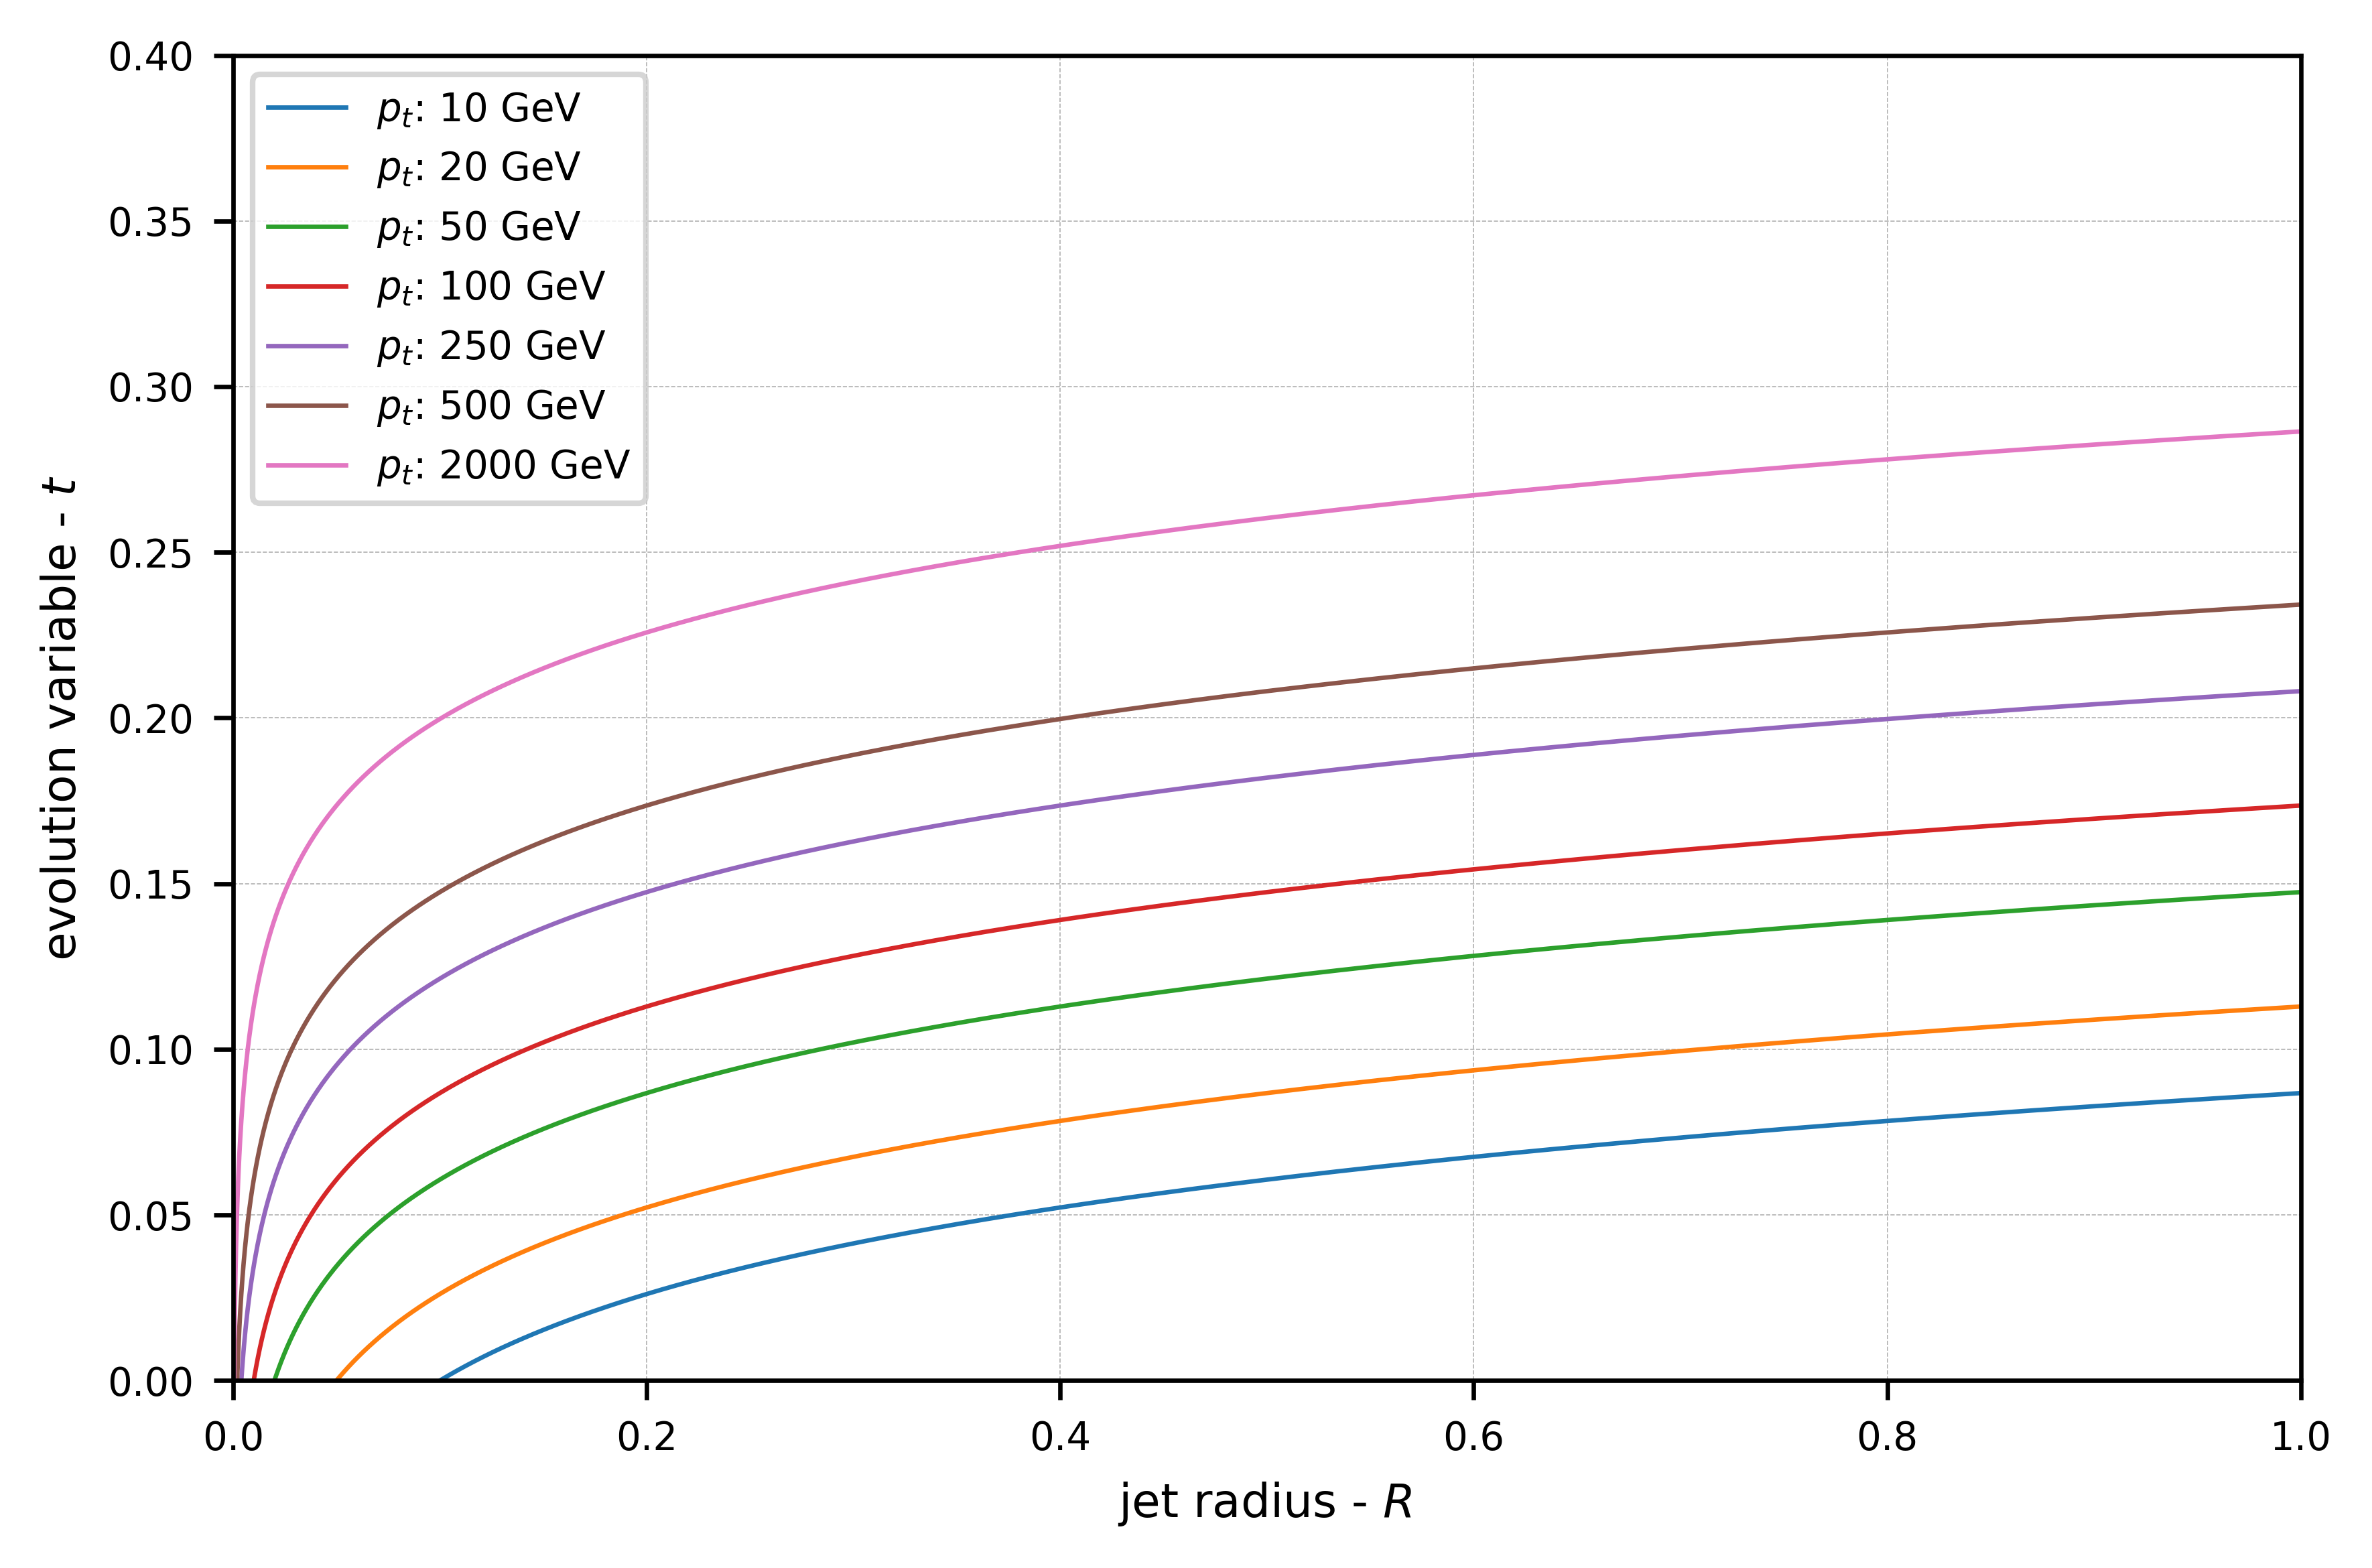
\includegraphics[width=9cm]{pictures/plots/misc/evolution_variable_vacuumshowers.png}
    \caption{Maximum values of the evolution variable \(t\) for vacuum showers, plotted up to \(p_t\,R > Q_0\). The strong coupling is set to be constant \(\alpha_S = 0.1184\), and hadronization scale \(Q_0 = 1 GeV\).}
    \label{fig: evolution_variable_vacuumshowers}
\end{figure}

Knowing the boundaries we need to impose on the evolution parameter for our MC, we can now move on to determining how to sample intervals of the evolution parameter.
This can be done using the Sudakov form factor - which is related to the branching probability - to randomly determine an interval \(\Delta t\) in which we can expect a branching. This is because the probability of no branching in the interval \([t_0, t]\), is given directly from the Sudakov form factor introduced in \autoref{eqn: sudakov_form_factor_dasguptalike},
\begin{equation}\label{eqn: branching_probability_from_sudakov_gg}
    \mathcal{P}(\Delta t) = \frac{\Delta(t)}{\Delta(t_0)} = \exp\left(-\Delta t \int_\epsilon^{1-\epsilon}dz \, P_{gg}(z)\right) 
\end{equation}
Therefore, we can generate a random number in the interval \(\mathcal{P}(\Delta t) = \mathcal{R} \in [0,1]\), and use it to solve for \(\Delta t\), at which we can expect to get a new splitting, 
%\begin{equation*}
%    \mathcal{R} = exp\left(-\Delta t \int_\epsilon^{1-\epsilon}dz \, P_{gg}(z)\right) 
%\end{equation*}
\begin{equation}\label{eqn: expected_branching_interval}
    \Delta t = -\frac{ln(\mathcal{R})}{ \int_\epsilon^{1-\epsilon}dz \, P_{gg}(z)} 
\end{equation}
Therefore, in our Monte-Carlo, the evolution boundaries will be implemented as given in \autoref{alg: evolution_boundaries},
\begin{center}
\begin{minipage}{.8\linewidth}
\begin{algorithm}[H]
\caption{Evolution boundaries}
\label{alg: evolution_boundaries}
\begin{algorithmic}[1]
    \State calculate \(t_{\text{max}}\),
         \[t_{\text{max}} = \frac{\alpha_S}{\pi} \ln \frac{Rp_t}{Q_0}\]
    \While{\(t< t_{\text{max}}\)}
        \For{parton \textbf{in} AllPartons}
        \State calculate expected splitting interval. \[\Delta t = -\frac{ln(\mathcal{R})}{ \int_\epsilon^{1-\epsilon}dz \, P_{gg}(z)}\]
        \EndFor
    \State select the parton with shortest interval, \(\Delta t_{\text{min}} = \text{min}(\Delta t)\)
    \State evolve the angle \(t = t + \Delta t_{\text{min}}\).
    \EndWhile
\end{algorithmic}
\end{algorithm}
\end{minipage}
\end{center}

The general method outlined here is valid for all the vacuum programs, but \autoref{eqn: expected_branching_interval} is only valid for \(gg\)-branchings.

\subsection{Managing quarks and gluons}\label{sec: managing_quarks_and_gluons}
When creating a program with both quarks and gluons, we need to evolve the interval based on which kind of parton we are splitting. When splitting a gluon the interval will evolve according to the Sudakov given in \autoref{eqn: sudakov_vacuum_gluons}, and when splitting quarks the Sudakov is \autoref{eqn: sudakov_vacuum_quarks}. The branching probabilities are then calculated from the following equations,
\begin{align}
    \mathcal{P}_{g}(\Delta t) &= \exp\left(-\Delta t \int_\epsilon^{1-\epsilon} P_{qg}(z) + P_{gg}(z) \, dz \right)  \label{eqn: sudakov_splitting_interval_gluons}  \\
    \mathcal{P}_{q}(\Delta t) &= \exp\left(-\Delta t \int_\epsilon^{1-\epsilon} P_{qq}(z) \, dz \right) \label{eqn: sudakov_splitting_interval_quarks}
\end{align}
As mentioned above, we will branch the parton which gives to lowest value for \(\Delta t\). The question that remains is how to determine the splitting vertex when this parton is a gluon. This can be done by comparing the contribution of the two vertices have on the available phase space.
\begin{equation}\label{eqn: gluon_splitting_selection_ratios}
    W_{gg} = \frac{\int_\epsilon^{1-\epsilon} P_{gg}(z) \, dz}{\int_\epsilon^{1-\epsilon}P_{qg}(z) + P_{gg}(z) \, dz}
\end{equation}
If the splitting parton is a gluon, we need to roll a random number\(\mathcal{R}\in[0,1)\), if the value \(\mathcal{R}< W_{gg}\), we will use the \(gg\) vertex, and if \(\mathcal{R}\geq W_{gg}\) it will be the \(qg\) vertex. When setting \(\epsilon = 10^{-3}\), the value is \(W_{gg} \approx 0.96\), so the vast majority of gluon splittings will be done via the \(gg\) vertex.

A similar comparison could have been done for the relative contributions on the total phase space for quarks and gluons, but this is already implemented into the calculations for \(\mathcal{P}_q(\Delta t)\), and \(\mathcal{P}_g(\Delta t)\), so this is not necessary. 


\subsection{Sampling from the vacuum splitting functions}\label{sec: metropolis_hastings}
Now, that we know at what evolution interval we can expect to get a branching and how to select quarks or gluons to branch, we must determine the momentum fraction carried by the branched partons.
This can be done if we consider the probability density given as,
\begin{equation}\label{eqn: probability_density_for_splitting}
    \mathcal{P}(z) = \frac{ P_{ba}(z)}{\int_\epsilon^{1-\epsilon} dz \, P_{ba}(z)}
\end{equation}
which means that we can generate random momentum fractions for the branched parton, to be equal the distribution of \eqref{eqn: probability_density_for_splitting}, by the following relation,
\begin{equation}\label{eqn: energyfraction_function_R}
    \mathcal{R} \cdot \int_\epsilon^{1-\epsilon} dz \, P_{ba}(z) = \int_\epsilon^{y}dz \, P_{ba}(z)
\end{equation}
where \(\mathcal{R}\in [0,1]\) \cite{ellis_stirling_webber_1996}. Note that since the splitting function is present on both sides of the equation, we can disregard any color and symmetry factors when calculating the splitting value, as they will not impact the final sample.

When trying to solve \autoref{eqn: energyfraction_function_R} for the different splitting functions, we will find that not all of them can be solved for a general momentum-fraction \(y\), and we need to introduce the Metropolis-Hastings algorithm for sampling them correctly \cite{MCMC_andrieu2003}.

The Metropolis-Hastings algorithm requires two different distributions,
\begin{itemize}
    \item A target distribution \(P(x)\), which is the one we are trying to sample.
    \item A proposal distribution \(f(x)\) proportional to \(\mathcal{P}(x)\).
\end{itemize}
Once these are chosen the Metropolis-Hastings algorithm is executed according to \autoref{alg: metropolis_hastings},
\begin{center}
\begin{minipage}{.8\linewidth}
\begin{algorithm}[H]
\caption{Metropolis-Hastings}
\label{alg: metropolis_hastings}
\begin{algorithmic}[1]
    \State sample a random value \(x'\) from \(f(x)\).
    \State calculate the acceptance probability, \[A(x') = \text{min} \left(1, \, \frac{P(x')}{f(x')}\right)\]
    \State generate a random number \(\mathcal{R}\in [0,1]\).
    \If{\(\mathcal{R}\leq A(x')\)} 
        \Statey accept the value \(x = x'\)
    \ElsIf{\(\mathcal{R} > A(x')\)} 
        \Statey reject the value \(x'\)
    \EndIf
\end{algorithmic}
\end{algorithm}
\end{minipage}
\end{center}

We will now use \autoref{eqn: energyfraction_function_R} to sample random energy fractions, proportionally to the full splitting functions as derived in \autoref{sec: derivation_splitting_functions_vacuum}.

\subsubsection*{Sampling from the \(gg\) vertex}
When trying to solve \autoref{eqn: energyfraction_function_R} for the \(gg\) splitting function in \autoref{eqn: vacuum_gg_splitting_function}, we will see that it is difficult to solve for \(y\). We will therefore introduce a simplified splitting function, which can be used in the Metropolis-Hastings algorithm.
\begin{equation}\label{eqn: p_ggg_vacuum_dummy}
    P_{gg}^{\text{(dummy)}}(z) = \frac{1}{z(1-z)}
\end{equation}
And we then need to evaluate \autoref{eqn: energyfraction_function_R} to obtain a way of sampling values from this simplified splitting function. The integral is straightforward to execute,
\begin{align}
    \mathcal{R} \int_\epsilon^{1-\epsilon} dz \, \frac{1}{z(1-z)} &= \int_\epsilon^{y} \frac{1}{z(1-z)}  \nonumber\\
    \mathcal{R} \left(  \ln (\frac{1-\epsilon}{\epsilon}) + ln(\frac{1-\epsilon}{\epsilon}) \right) &= \ln (\frac{y}{1-y}) + ln(\frac{1-\epsilon}{\epsilon}) \nonumber\\
    \mathcal{R} \cdot 2 \left( \ln (\frac{1-\epsilon}{\epsilon}) \right) &= \ln (\frac{y}{1-y} \cdot \frac{1-\epsilon}{\epsilon})
\end{align}
exponentiating both sides, 
\begin{align}\label{eqn: MC_energyfraction_origin_vacuum}
    \frac{y}{1-y} \frac{1-\epsilon}{\epsilon} &= \left(\frac{1-\epsilon}{\epsilon}\right)^{2\cdot \mathcal{R}} \nonumber\\
    \frac{y}{1-y} &= \left(\frac{1-\epsilon}{\epsilon}\right)^{(2\cdot \mathcal{R}-1)} \nonumber\\
    y &= \frac{\left(\frac{1-\epsilon}{\epsilon}\right)^{(2\cdot \mathcal{R}-1)}}{1+\left(\frac{1-\epsilon}{\epsilon}\right)^{(2\cdot \mathcal{R}-1)}}
\end{align}
simplifying the expression we obtain \autoref{eqn: MC_energyfraction_gg_vacuum} which can be used to randomly generate parton energy fractions, 
\begin{equation}\label{eqn: MC_energyfraction_gg_vacuum}
    y(\mathcal{R}) = \frac{\xi}{1+ \xi} \qquad \text{for, } \quad \xi = \left(\frac{1-\epsilon}{\epsilon}\right)^{(2\cdot \mathcal{R}-1)}
\end{equation}

%Histogram for the randomly sampled dummy splitting function values compared to the exact dummy splitting functions is plotted in \autoref{fig: function_vs_MC_simplified_pgg_splitting}. It is therefore apparent that \autoref{eqn: MC_energyfraction_gg_vacuum} is a valid method for sampling random energy fractions from the distribution given by the dummy splitting function.
%\begin{figure}[htb]
%    \centering
%    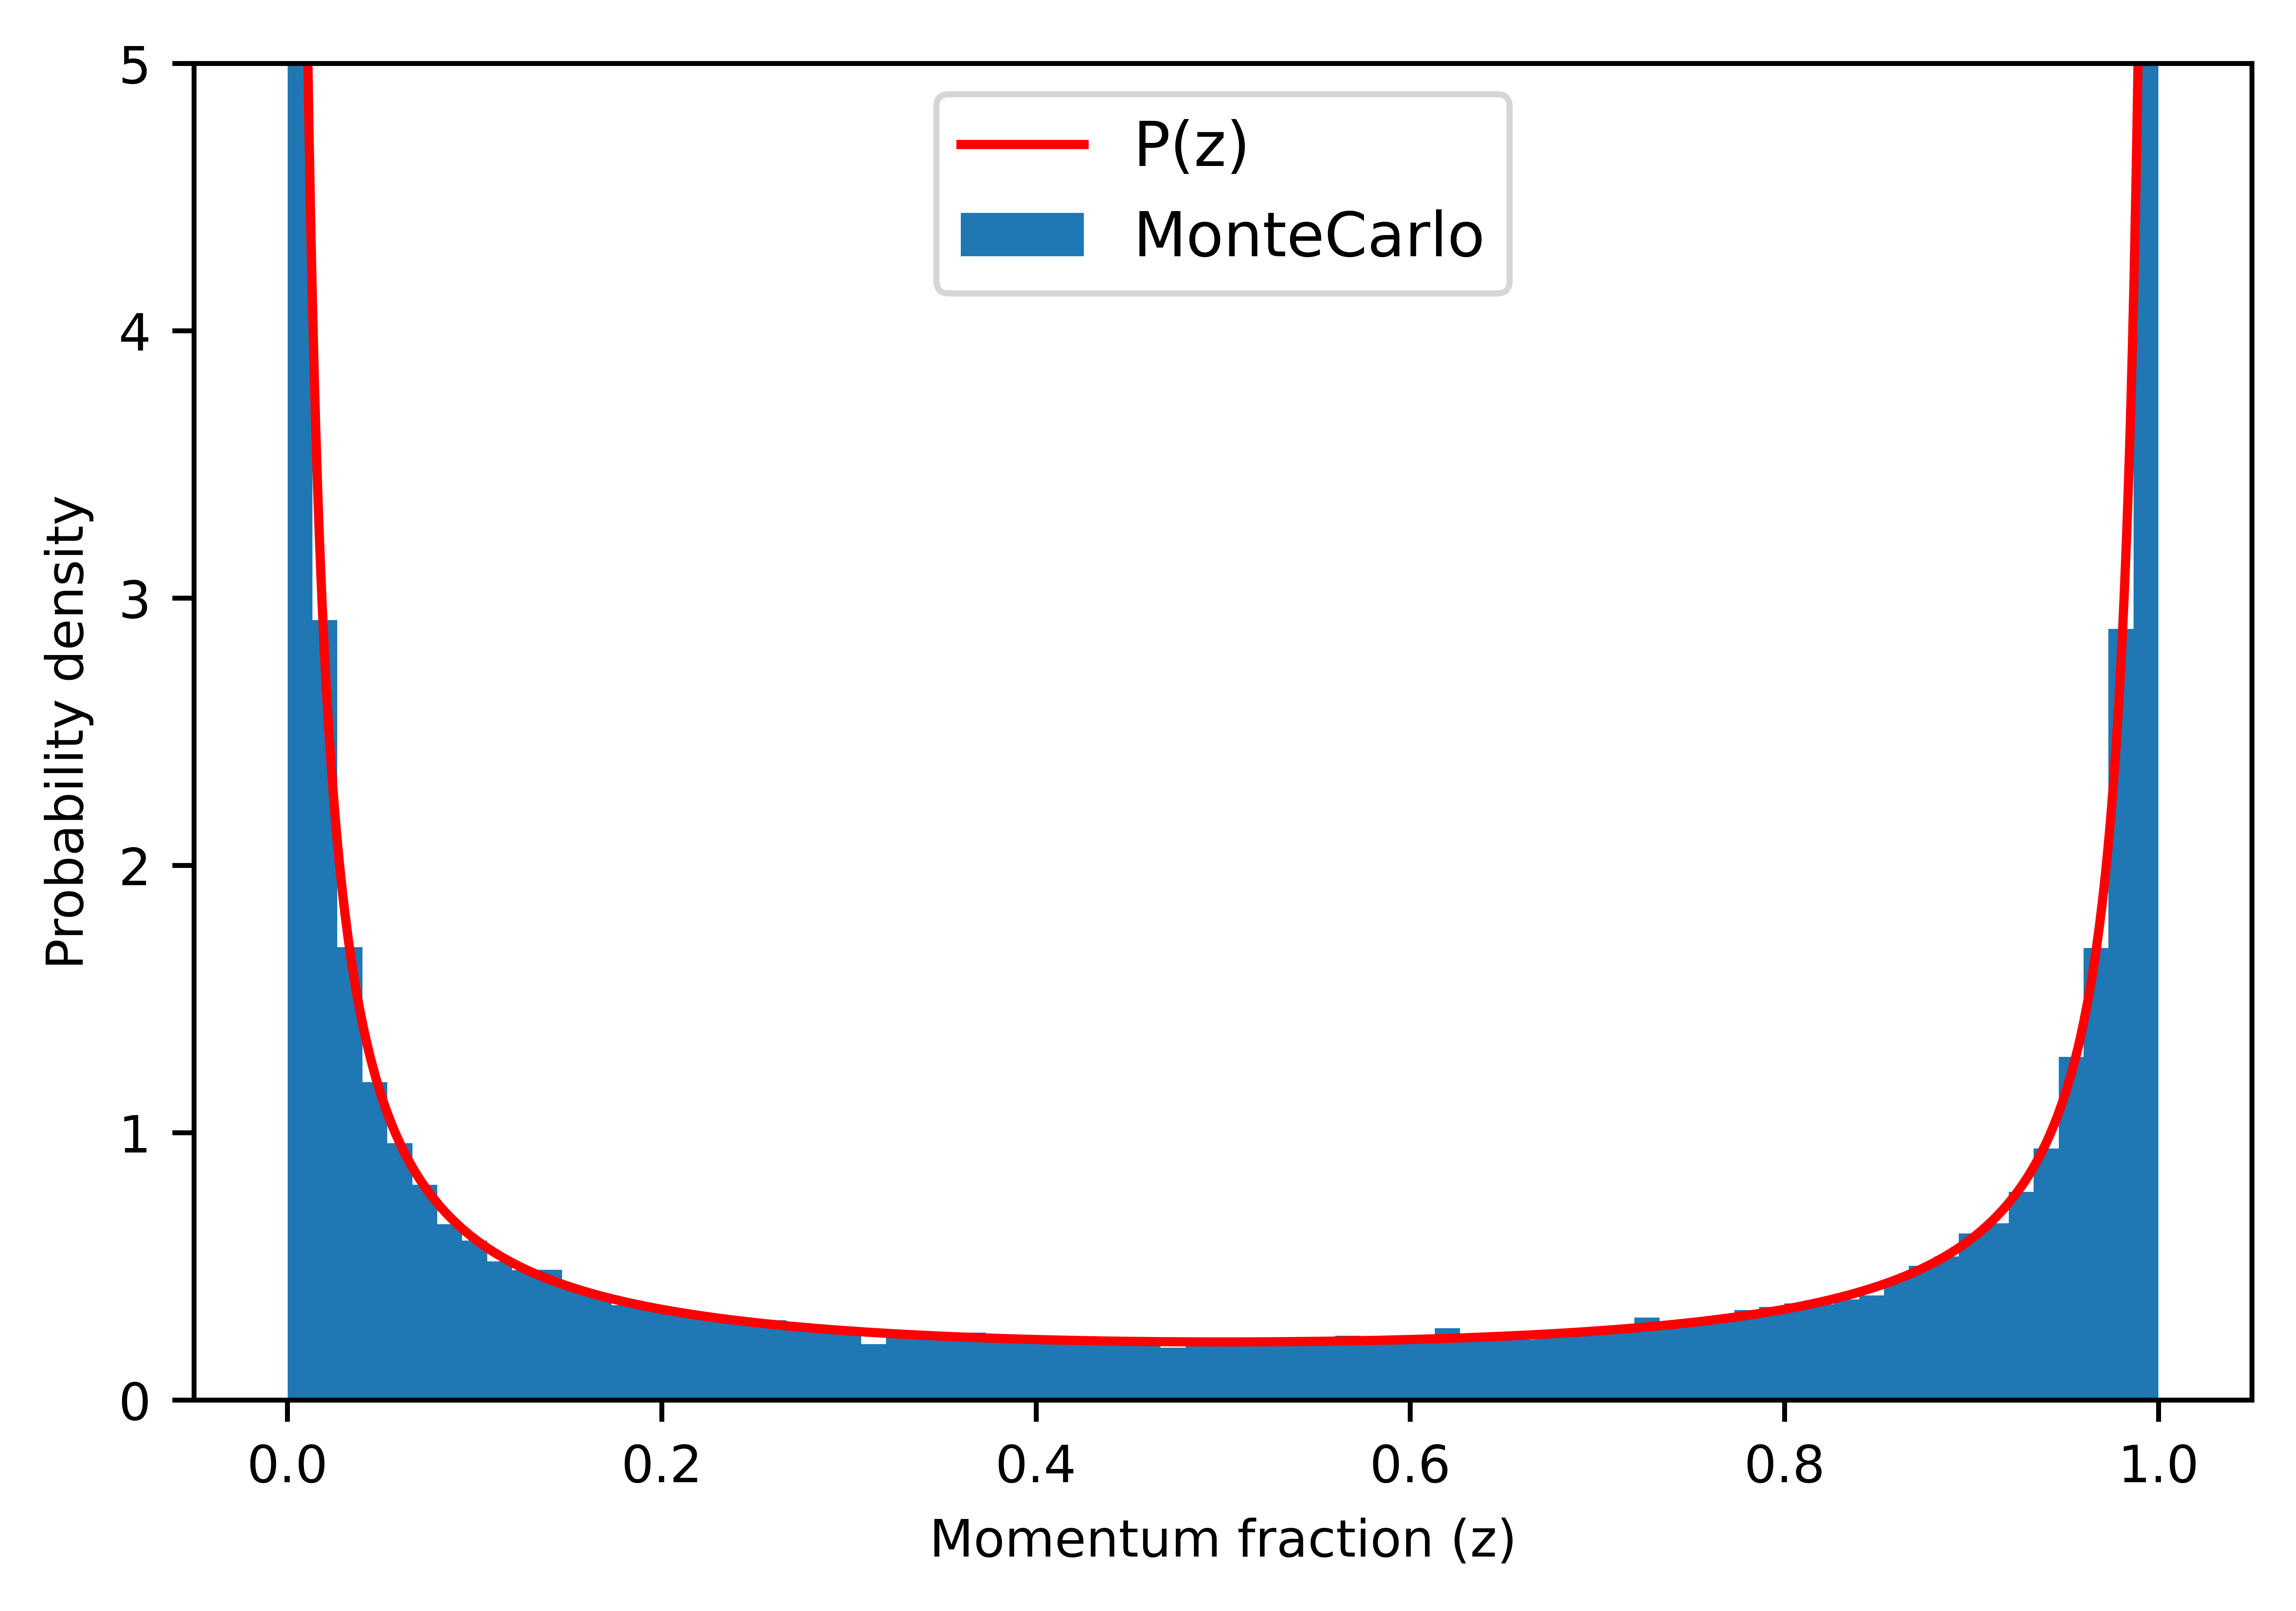
\includegraphics[width=7cm]{pictures/plots/Metropolis-Hastings/p_ggg_simple_MCvsPZ.png}
%    \caption{Probability density for momentum fractions vs density histogram of randomly generated momentum fractions for a simplified \(P_{gg}\) splitting function. Generated with \(100,000\) points.\krs{remove this}}
%    \label{fig: function_vs_MC_simplified_pgg_splitting}
%\end{figure}

Applying the Metropolis-Hastings algorithm by using the dummy splitting function sampling determined by \autoref{eqn: MC_energyfraction_gg_vacuum}, we can generate a plot of the original histogram, compared to the Metropolis-Hastings correction. This gives us a good idea of how the correction works, and allows us to demonstrate how this simple algorithm allows us to sample more complex functions. The resulting plot is given in \autoref{fig: MH_corrected_p_gg_splitting}.
\begin{figure}[htb]
    \centering
    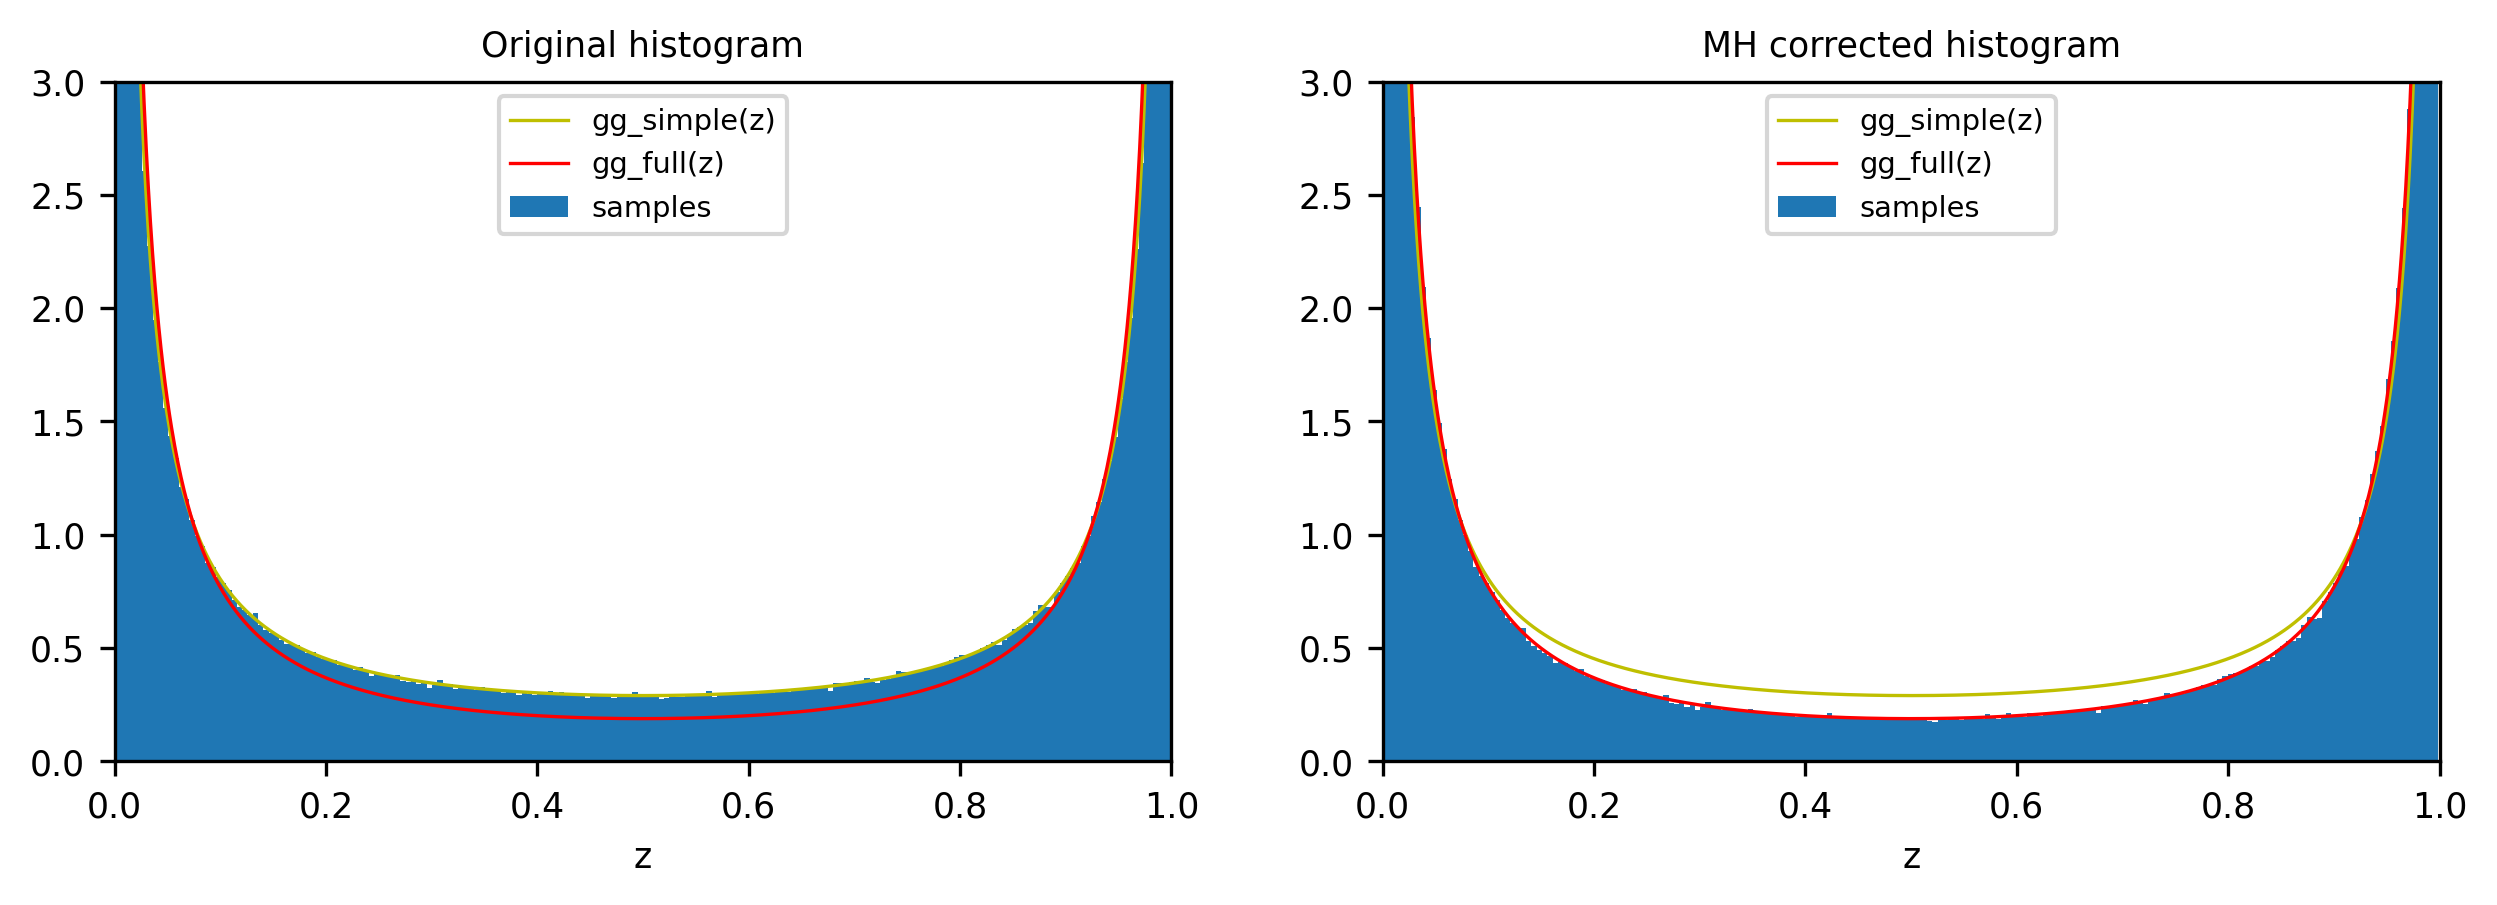
\includegraphics[width=15cm]{pictures/plots/Metropolis-Hastings/MH_vacuum_gg.png}
    \caption{Probability density of the full \(P_{gg}\) splitting function, compared to the density histogram of the dummy splitting function, and the Metropolis-Hastings corrected results. Simulated with \(1,000,000\) points, and an acceptance rate of \(0.87\).}
    \label{fig: MH_corrected_p_gg_splitting}
\end{figure}

\subsubsection*{Sampling from the \(qg\) vertex}
Now we will find a way of sampling random values from the \(qg\) splitting function given by \autoref{eqn: vacuum_qg_splitting_function}. In contrast to the other splitting functions, this one is actually not divergent, so we can set \(\epsilon = 0\). 

Solving the integrals, \autoref{eqn: energyfraction_function_R} becomes,
\begin{align}
    \mathcal{R} \cdot \frac{2}{3} &= \left[ y - y^2 + \frac{2}{3} y^3 \right] \nonumber\\
    \mathcal{R} \cdot \frac{2}{3} &= y - y^2 + \frac{2}{3} y^3 \nonumber \\
    0 &= \frac{2}{3} y^3 - y^2 + y - \frac{2\mathcal{R}}{3} \label{eqn: gqq_vertex_qubic_formula}
\end{align}
This is cubic formula. Setting \(d = (\frac{2\mathcal{R}}{3}) \), we can throw \autoref{eqn: gqq_vertex_qubic_formula} into WolframAlpha, and find the single real root to be,
\begin{equation}\label{eqn: gqq_vacuum_sample}
    y \approx 0.5 + 0.5 \cdot((36 d^2 - 24 d + 5)^{1/2} + 6 d - 2)^{1/3} - \frac{0.5}{((36 d^2 - 24 d + 5)^{1/2} + 6 d - 2)^{1/3}}
\end{equation}
It is therefore possible to sample randomly without using the Metropolis-Hastings algorithm. An argument could be made that it takes more time for python to calculate the value of this polynomial, than it would to generate a MH corrected value from a simpler function, but this allows for some interesting variation in how we determine our splitting values. The histogram of random samples generated, versus the exact splitting density is given by \autoref{fig: p_qg_splitting}.
\begin{figure}[htb]
    \centering
    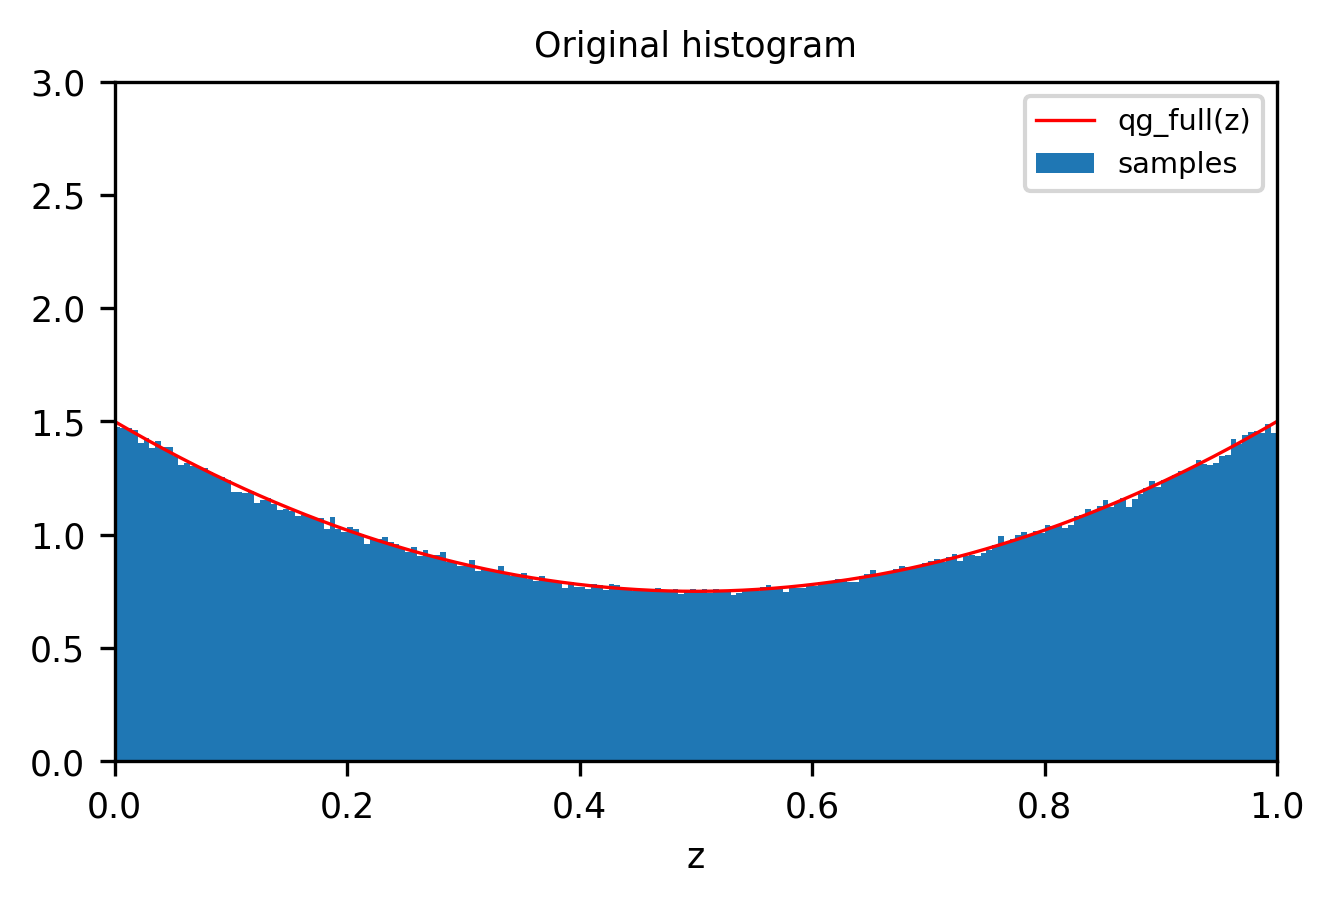
\includegraphics[width=9cm]{pictures/plots/Metropolis-Hastings/MH_vacuum_qg.png}
    \caption{Probability density of the full \(\hat{P}_{qg}\) splitting function, compared to the histogram of 1,000,000 generated samples.}
    \label{fig: p_qg_splitting}
\end{figure}

\subsubsection*{Sampling from the \(qq\) vertex}
Next up we will solve \autoref{eqn: energyfraction_function_R} for the \(qq\) splitting function of \autoref{eqn: vacuum_qq_splitting_function}.
\begin{align}
    \int dz\hat{P}_{qq}(z) &= \int \left(\frac{1+z^2}{1-z} \right)\, dz \nonumber \\
    &= \int \left(\frac{-(z^2+1)}{z-1} \right)\, dz \nonumber \\
    &= \int \left(\frac{-((z-1)(z-1)+2z)}{z-1} \right)\, dz \nonumber \\
    &= \int -(z-1)\, dz - \int \frac{2z}{z-1} \, dz \nonumber \\
    &= \int (1-z) \, dz - \int \frac{2(u+1)}{u} \, du \qquad \text{, where}\; u=z-1 \nonumber \\
    &= \int (1-z) \, dz - \int 2\, dz - \int_a^b \frac{2}{u} \, du \nonumber  \\
    &= -\int (z+1) \, dz - \int \frac{2}{u} \, du \nonumber  \\
    &= -\frac{z^2}{2} - z - 2\left( ln(z-1)\right) 
\end{align}
since this integral has an exact solution, we can solve \autoref{eqn: energyfraction_function_R} for this splitting function,

\begin{align}
    \mathcal{R} \cdot \left[-\frac{z^2}{2} - z - 2\left( ln(z-1)\right) \right]_\epsilon^{1-\epsilon} &= \left[-\frac{z^2}{2} - z - 2\left( ln(z-1)\right) \right]_\epsilon^{y} \nonumber \\
    %\mathcal{R} \cdot \left(-\frac{(1-\epsilon)^2}{2} - (1-\epsilon) - 2 ( ln((1-\epsilon)-1)) \right) &- \mathcal{R} \cdot \left( -\frac{\epsilon^2}{2} - \epsilon - 2 ( ln(\epsilon-1)) \right) \nonumber \\
    %&= \left(-\frac{y^2}{2} - y - 2 ( ln(y-1)) \right) - \left( -\frac{\epsilon^2}{2} - \epsilon - 2 ( ln(\epsilon-1)) \right) \nonumber
    \mathcal{R}\cdot|  \frac{6 \epsilon-3}{2} - 2 ( ln(-\epsilon)) + 2 ( ln(\epsilon-1)) &= -\frac{y^2}{2} - y - 2 ( ln(y-1)) +\frac{\epsilon^2}{2} + \epsilon + 2 ( ln(\epsilon-1)) \nonumber\\
    \frac{y^2}{2} + y + \ln \left( \frac{y-1}{\epsilon-1}\right)^2  &= -\left(\mathcal{R} \cdot \frac{6 \epsilon-3}{2} + \frac{-\epsilon^2-4 \epsilon}{2}\right) - ln\left(\frac{1-\epsilon}{\epsilon}\right)^{2\mathcal{R}}
\end{align}
This equation is however difficult to solve, so we will need to use the Metropolis-Hastings algorithm once again. The \(qq\) splitting function is \(\hat{P}_{qq}(z) = \frac{1+z^2}{1-z}\), we will try a dummy function \(\hat{P}_{qq}^{\text{dummy}} = \frac{-2}{z-1}\). The integral of his dummy function is simply,
\begin{align}
    \int(\frac{-2}{z-1})dz = -2 ln(z-1)
\end{align}
Now we will try to solve \autoref{eqn: energyfraction_function_R}, with this dummy splitting function, 
\begin{align}
    \mathcal{R}\cdot \left[-2 ln(z-1)\right]_{\epsilon}^{1-\epsilon} &= \left[-2 ln(z-1)\right]_{\epsilon}^{y} \nonumber \\
    \mathcal{R}\cdot \left(-2 ln((1-\epsilon)-1) + 2 ln(\epsilon-1) \right) &= \left(-2 ln(y-1) + 2 ln(\epsilon-1) \right) \nonumber \\
    \mathcal{R}\cdot ln\left(\frac{1-\epsilon}{\epsilon} \right) &= - ln(y-1) + ln(\epsilon-1)
\end{align}
moving terms and exponentiating, 
\begin{align}
    ln(y-1) &= ln(\epsilon-1) - ln\left(\frac{1-\epsilon}{\epsilon} \right)^{\mathcal{R}} \nonumber \\
    y-1 &= \frac{e^{ln(\epsilon-1)}}{e^{ln(\frac{1-\epsilon}{\epsilon})^{\mathcal{R}}}} \nonumber \\
    y &= \frac{(\epsilon-1)}{(\frac{1-\epsilon}{\epsilon})^{\mathcal{R}}} +1 
\end{align}
This equation can be used for sampling random values from the simple \(qq\) splitting function, and following the same procedure as in Section \ref{sec: metropolis_hastings} we can implement Metropolis-Hastings algorithm for sampling random values from the full \(qq\) splitting function. The results of both the original samples, and the MH corrected histogram is given in \autoref{fig: MH_corrected_p_qq_splitting}.
\begin{figure}[htb]
    \centering
    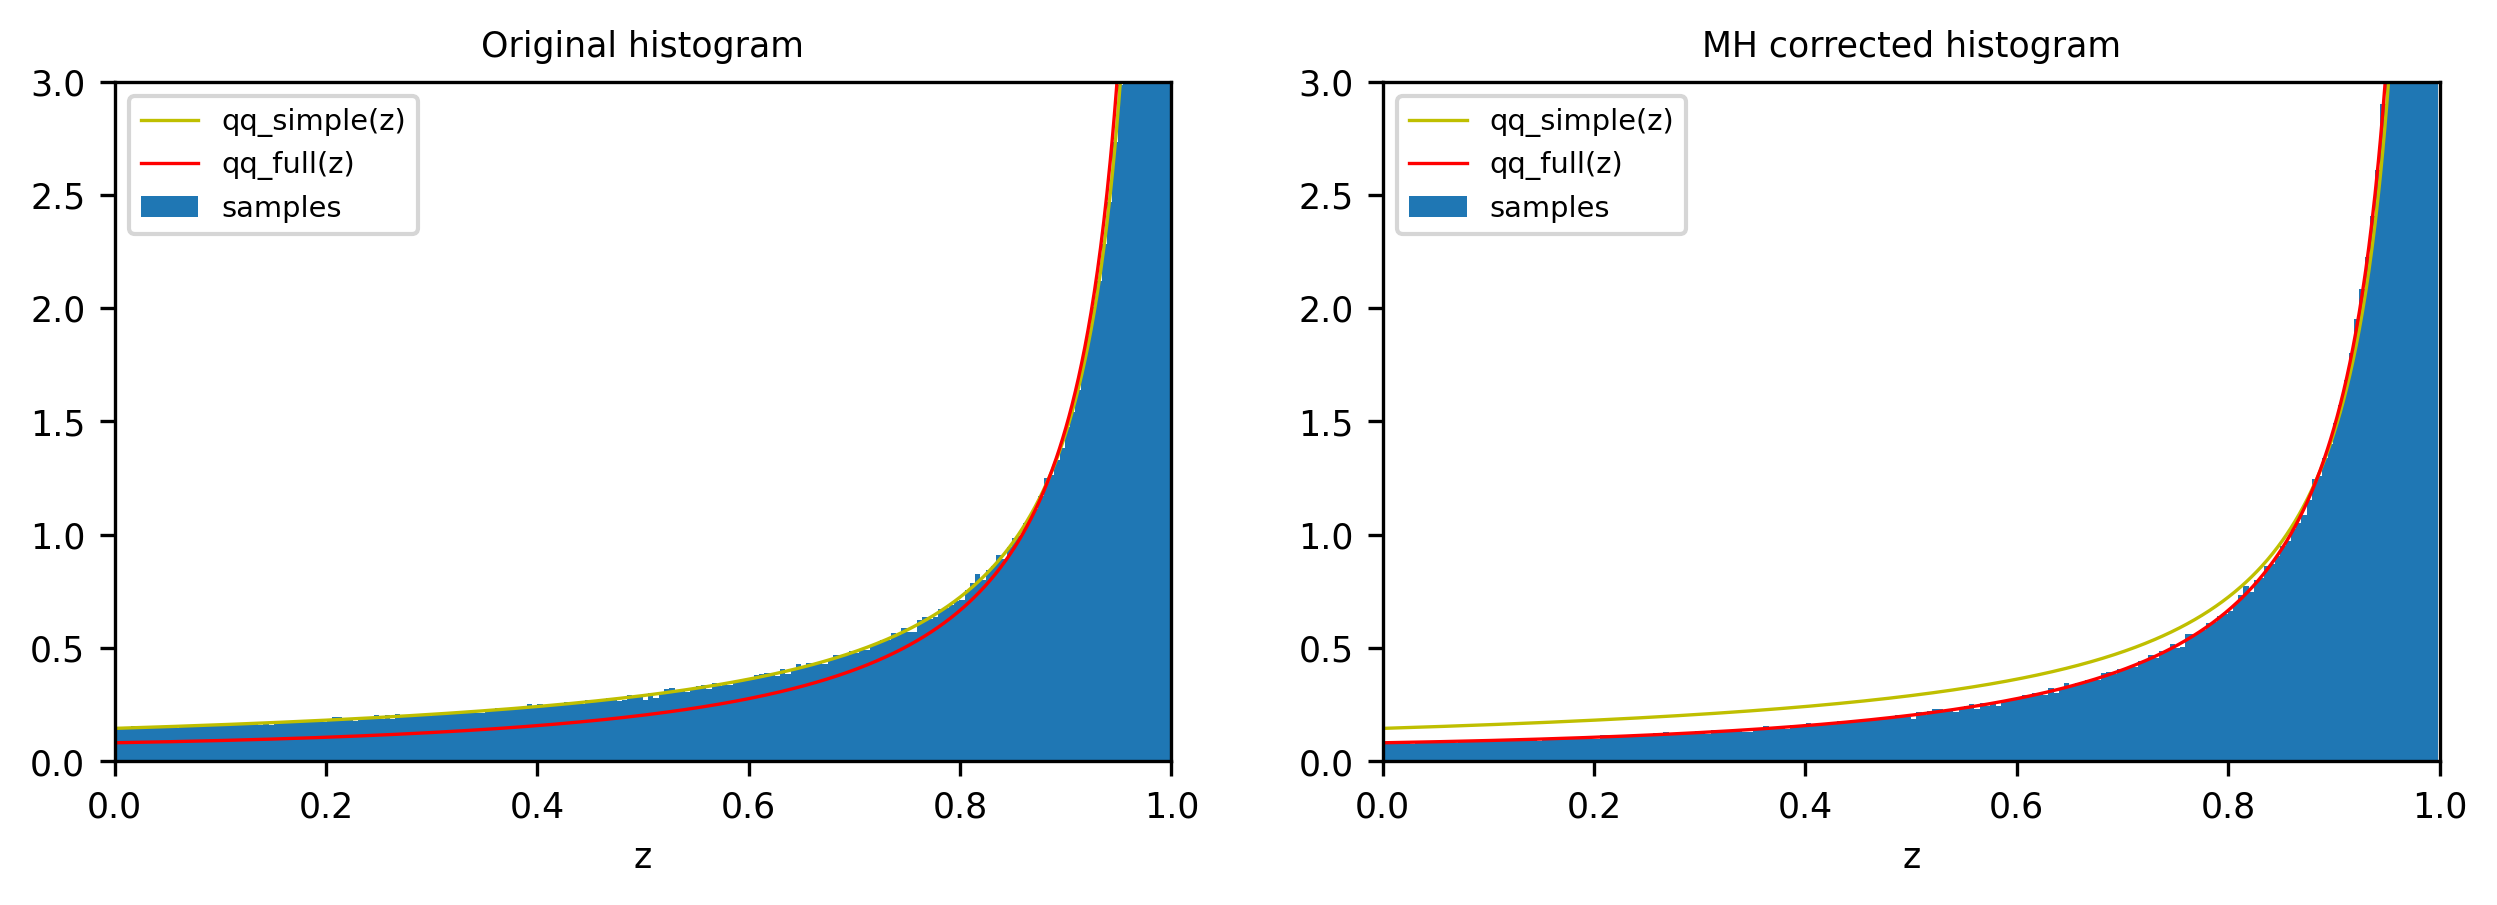
\includegraphics[width=15cm]{pictures/plots/Metropolis-Hastings/MH_vacuum_qq.png}
    \caption{Probability density of the full \(\hat{P}_{qq}\) splitting function, compared to the density histogram of the dummy splitting function, and the Metropolis-Hastings corrected results. Simulated with \(1,000,000\) points, and an acceptance rate of \(0.89\).}
    \label{fig: MH_corrected_p_qq_splitting}
\end{figure}

\subsection{Monte-Carlo implementation}
This section serves to give a brief overview of the logical structure of the main \textit{generate\_shower} subprogram, which is the core of the parton-shower programs. This is where all of the actual physics is applied, while the rest of the program is for plotting, defining variables, and creating the \textit{PartonObject} and \textit{ShowerObject}. 

The full code for running the different parton shower programs, and Metropolis-Hastings algorithms is available on the authors GitHub \cite{GitHub_thesis}. The main loop running in the shower program is given here in \autoref{alg: generate_shower_loop}. Not all parameters are listed here, as to keep the representation as simple as possible.
\begin{center}
\begin{minipage}{.8\linewidth}
\begin{algorithm}[H]
\caption{generate\_shower main loop}
\label{alg: generate_shower_loop}
\begin{algorithmic}[1]
    \While{$ \text{len}(\text{SplittingPartons} > 0 $}
    \State SplittingParton, \(\Delta t\) = select\_splitting\_parton()
    \State \(t = t + \Delta t\)
    \State end\_shower = loop\_status(\(t, t_{\text{max}}\)) 
    \If{end\_shower}
        \State \textbf{break}
        \EndIf
    \State SplittingPartons.remove(SplittingParton)
    \State FinalList.remove(SplittingParton)
    \State $z$ = SplittingParton.split()
    
    \For{j \textbf{in} range(0,2)}
        \If{j==0}
            \State NewParton = Parton(\(t, xz\))
        \ElsIf{j==1}
            \State NewParton = Parton(\(t, x (1-z)\))
            \EndIf
            \EndFor
    \State Shower0.FinalList.append(NewParton)
    \If{NewParton.InitialFrac > \(z_{\text{min}}\sim 0.001\)}
        \State SplittingPartons.append(NewParton)
        \EndIf
    \EndWhile
    \State \textbf{return} Shower
\end{algorithmic}
\end{algorithm}
\end{minipage}
\end{center}

\subsection{Results for gluons in vacuum}
Starting by looking at the results for the parton shower with only gluons in vacuum. The distribution for the inclusive energy distribution \(D(x,t)\) is given in \autoref{fig: vacuum_gluons_MCandAnalytical_comparison}. The MC results is plotted alongside the analytical solution to the DGLAP equation on the form \autoref{eqn: DGLAP_solution_energyflowmedium}, using the simplified splitting function, with \(C_A=1\). 
\begin{figure}[htb]
    \centering
    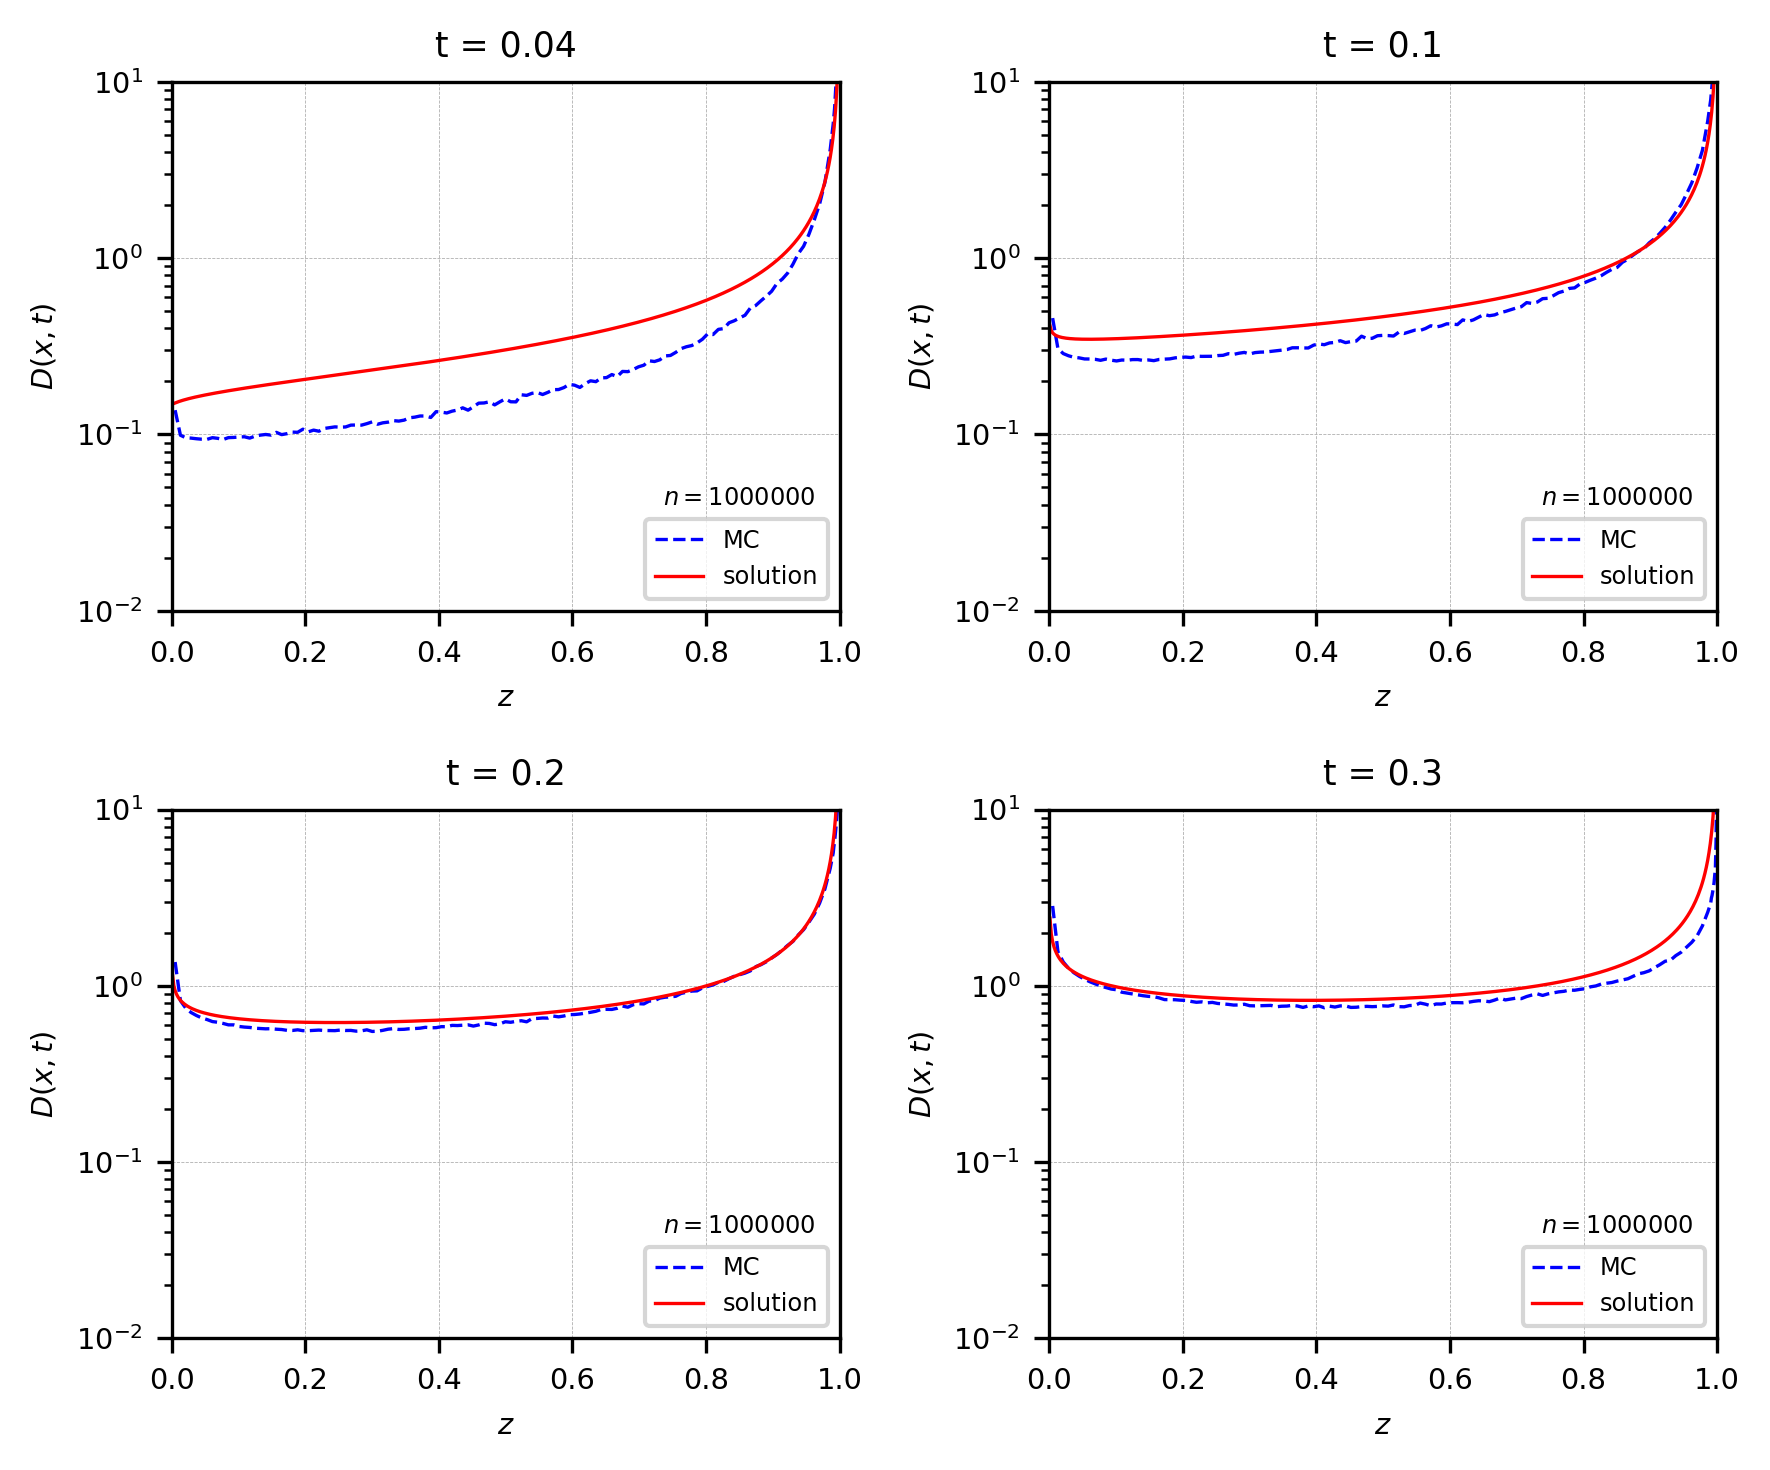
\includegraphics[width=12cm]{pictures/plots/distributions/vacuum/vacuum_shower_analytical_1m.png}
    \caption{Inlcusive distribution for \(n=10^6\) showers for gluons-only in vacuum, with the simplified splitting function ( \(C_A=1\)). Plotted alongside the analytical solution obtained in \autoref{eqn: branching_probability_from_sudakov_gg}. Parameters used are \(\epsilon=10^{-3}\) and \(z_{\text{min}}=10^{-3}\)}. 
    \label{fig: vacuum_gluons_MCandAnalytical_comparison}
\end{figure}

From \autoref{fig: vacuum_gluons_MCandAnalytical_comparison} it is apparent that the Monte-Carlo is in good agreement with the analytical solution for larger values of \(t\) - meaning when we are evolving with a parton with high initial \(p_t\). The discrepancies between the two graphs at lower values of \(t\) can be explained by \elab

\subsection{Results for quarks and gluons in vacuum}
Turning to the program with both quarks and gluons in vacuum. The resulting plot for the inclusive parton distribution \(f(x,t)\) as generated from our Monte-Carlo program for quarks and gluons in vacuum, is given in \autoref{fig: vacuum_distribution_quark_and_gluon}.
\begin{figure}[htb]
    \centering
    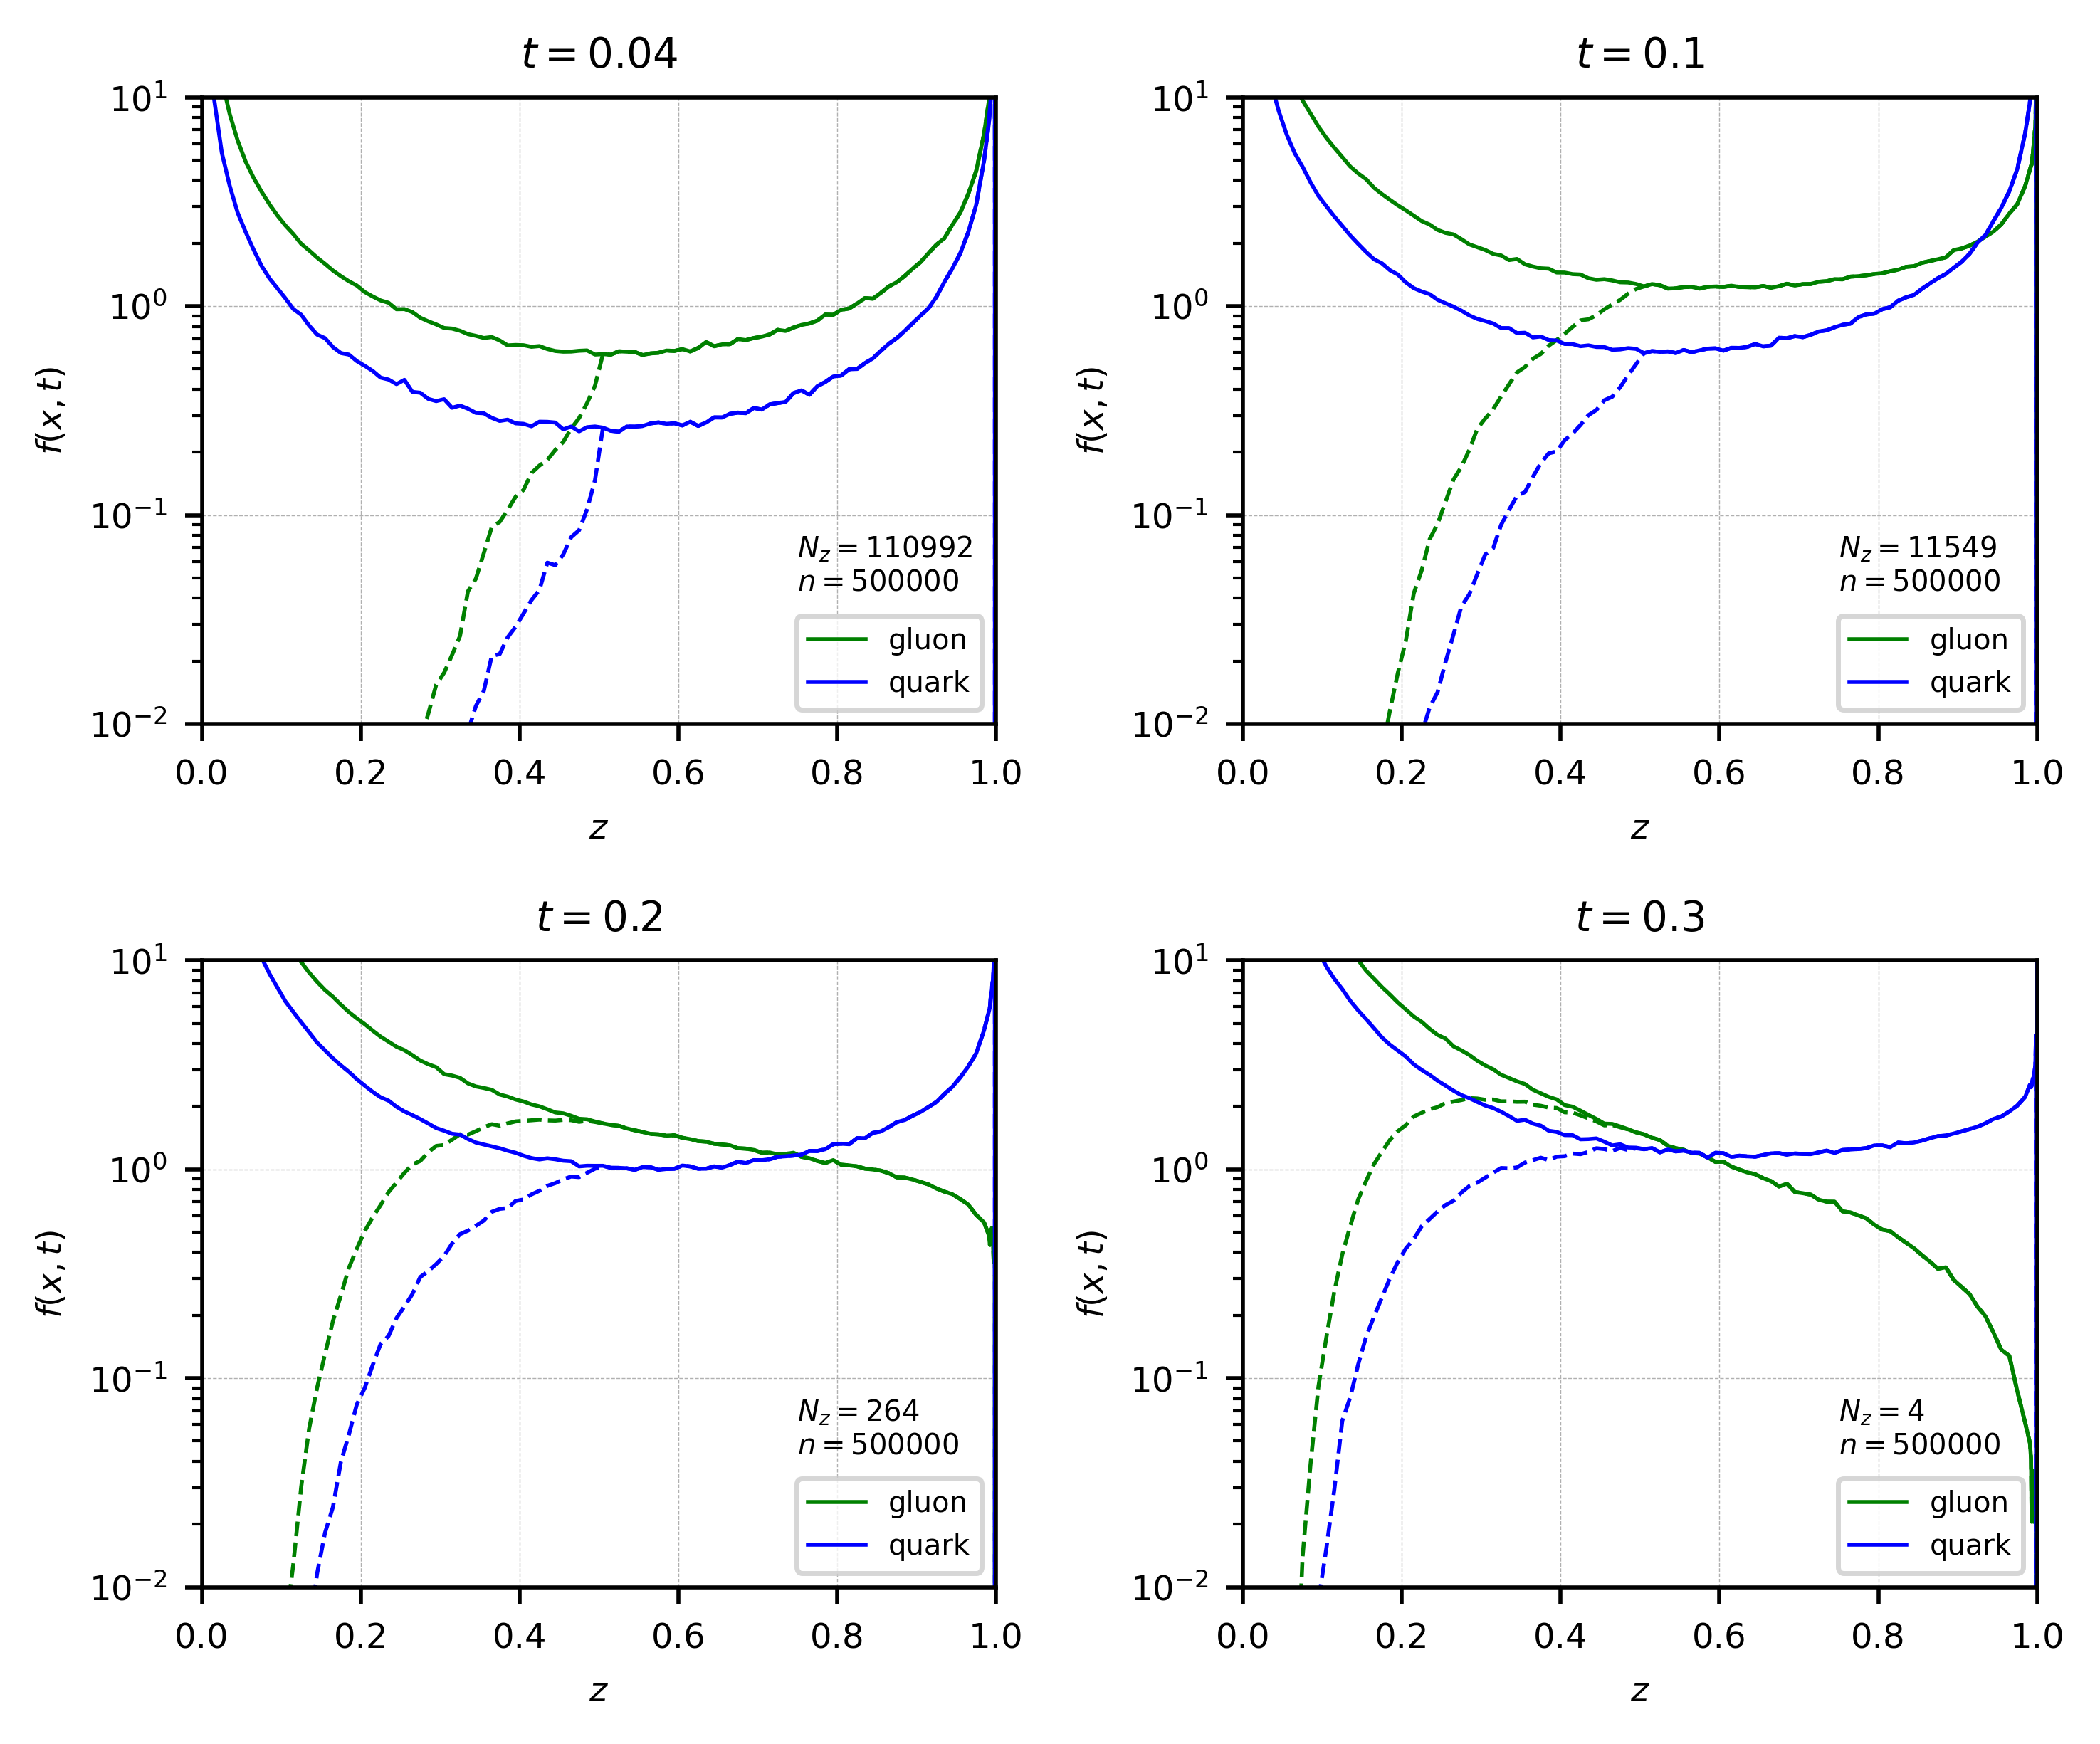
\includegraphics[width=12cm]{pictures/plots/distributions/vacuum/dasgupta_quarksgluons_N500000.png}
    \caption{Inclusive spectrum generated from the Monte-Carlo program with quarks and gluons in vacuum. The solid lines show the inclusive parton distribution for initial quarks (blue) and initial gluons (green). The dashed lines show the hardest parton of each shower. Simulated with \(n=5\cdot 10^5\) showers for both initial quark and initial gluon. Parameters used are \(\epsilon=10^{-3}\) and \(z_{\text{min}}=10^{-3}\). The number of gluons \(N_z\) with \(z=1\) is, \(N_z(0.04)=110992 \pm 157\), \(N_z(0.1)=11549.0 \pm 16.3\), \(N_z(0.2k)=264.0 \pm 0.4\), and \(N_z(0.3)=4.000 \pm 0.006\)}
    \label{fig: vacuum_distribution_quark_and_gluon}
\end{figure}

There are several observations to be made from this plot. Firstly the distribution of the hardest parton of each shower is the same as for the distribution of the full spectrum for values above \(z<\frac{1}{2}\). \krs{this is due to...}. 
Secondly...

An initial check of the validity of the program can be done by comparing with the results of \cite[Figure 2.]{Dasgupta_2015}, in which the inclusive distribution has been plotted for fixed values of the evolution variable, \(t=0.04, 0.1, 0.2, 0.3\). While \cite{Dasgupta_2015} discusses a slightly different approach, where the evolution goes from \(R<\theta<1\), meaning they obtain the total number of microjets within a given jet, as opposed to our treatment where we are looking for the parton distribution inside a jet with radius \(R\) such that, \(Q_0/p_t < \theta < R\). The result can however be compared as long as the evolution goes over the same effective angle, as is the case when we are plotting with the same values of \(t\). Our results is then in good agreement with \cite{Dasgupta_2015}.

More explicit calculations can be done for checking the validity of our results. From the DGLAP equation on integral form \autoref{eqn: DGLAP_evolutioneq_unregularized_integral_ellis}, there is a term \(\Delta(t)\, f(x,t_0)\), which represents the probability of no branchings to occur at all for the initial parton during the interval \(t\in[t_0, t_{max}]\). This can be calculated from \autoref{eqn: branching_probability_from_sudakov_gg}, except now we know the value of \(\Delta t\), and need to take into account the possibility of the gluon to branch into a \(gg\) or a \(q\bar q\)-pair. The probability is then given as,
\begin{equation}
    \mathcal{P}(t) = \exp \left(-t\, \int_{\epsilon}^{1-\epsilon}dz\, (P_{gg}(z) + P_{qg}(z)) \right)
\end{equation}
Using the same values for \(t\) and \(\epsilon=10^{-3}\) as in the plot, we find that 
\begin{align}\label{eqn: no_branching_sudakov_probability}
    \begin{split}
        \mathcal{P}(0.04) &\approx 2.22\cdot 10^{-1} \\
        \mathcal{P}(0.1) &\approx 2.32\cdot 10^{-2} \\
        \mathcal{P}(0.2)&\approx 5.40\cdot 10^{-4} \\
        \mathcal{P}(0.3) &\approx 1.25\cdot 10^{-5}
    \end{split}
\end{align}
These probabilities should manifest themselves in our plot, and we can find them by simply counting the number of partons \(N_z\) with momentum \(z=1\) in the final distribution for each value of \(t\). Running \(N=5\cdot 10^{5}\) showers, the percentages are as follows,
\begin{align}\label{eqn: no_branching_MC_probability}
    \begin{split}
        \mathcal{P}_{\text{MC}}(t=0.04) &= \frac{N_z(0.04)}{N} = \frac{110992}{5\cdot 10^{5}} \approx 2.22\cdot 10^{-1} \\
        \mathcal{P}_{\text{MC}}(t=0.1) &= \frac{N_z(0.1)}{N} = \frac{11549}{5\cdot 10^{5}} \approx 2.31\cdot 10^{-2} \\
        \mathcal{P}_{\text{MC}}(t=0.2) &= \frac{N_z(0.2)}{N} = \frac{264}{5\cdot 10^{5}} \approx 5.28\cdot 10^{-4} \\
        \mathcal{P}_{\text{MC}}(t=0.3) &= \frac{N_z(0.3)}{N} = \frac{4}{5\cdot 10^{5}} \approx 8\cdot 10^{-6}
    \end{split}
\end{align}
We can see that the probabilities given from the calculation of the Sudakov in \autoref{eqn: no_branching_sudakov_probability} is in reasonable good agreement for the probabilities we find when running \(5\cdot 10^5\) showers and counting \(N_z\) in \autoref{eqn: no_branching_MC_probability}. 

It could be argued that these results are more accurate than the gluon-only cascade, as there is no reason for a gluon not to branch into a \(q\bar q\)-pair, although it is significantly less likely than a \(gg\)-pair \footnote{For our program only about \(\sim 4\%\) of the gluon branchings are \(g\rightarrow q\bar q\)}. It would therefore be interesting to compare the distributions from a pure gluon shower in vacuum, with a gluon initiated shower with both quarks and gluons in vacuum. The resulting plot is given in \autoref{fig: vacuum_program_comparisons}.
\begin{figure}[htb]
    \centering
    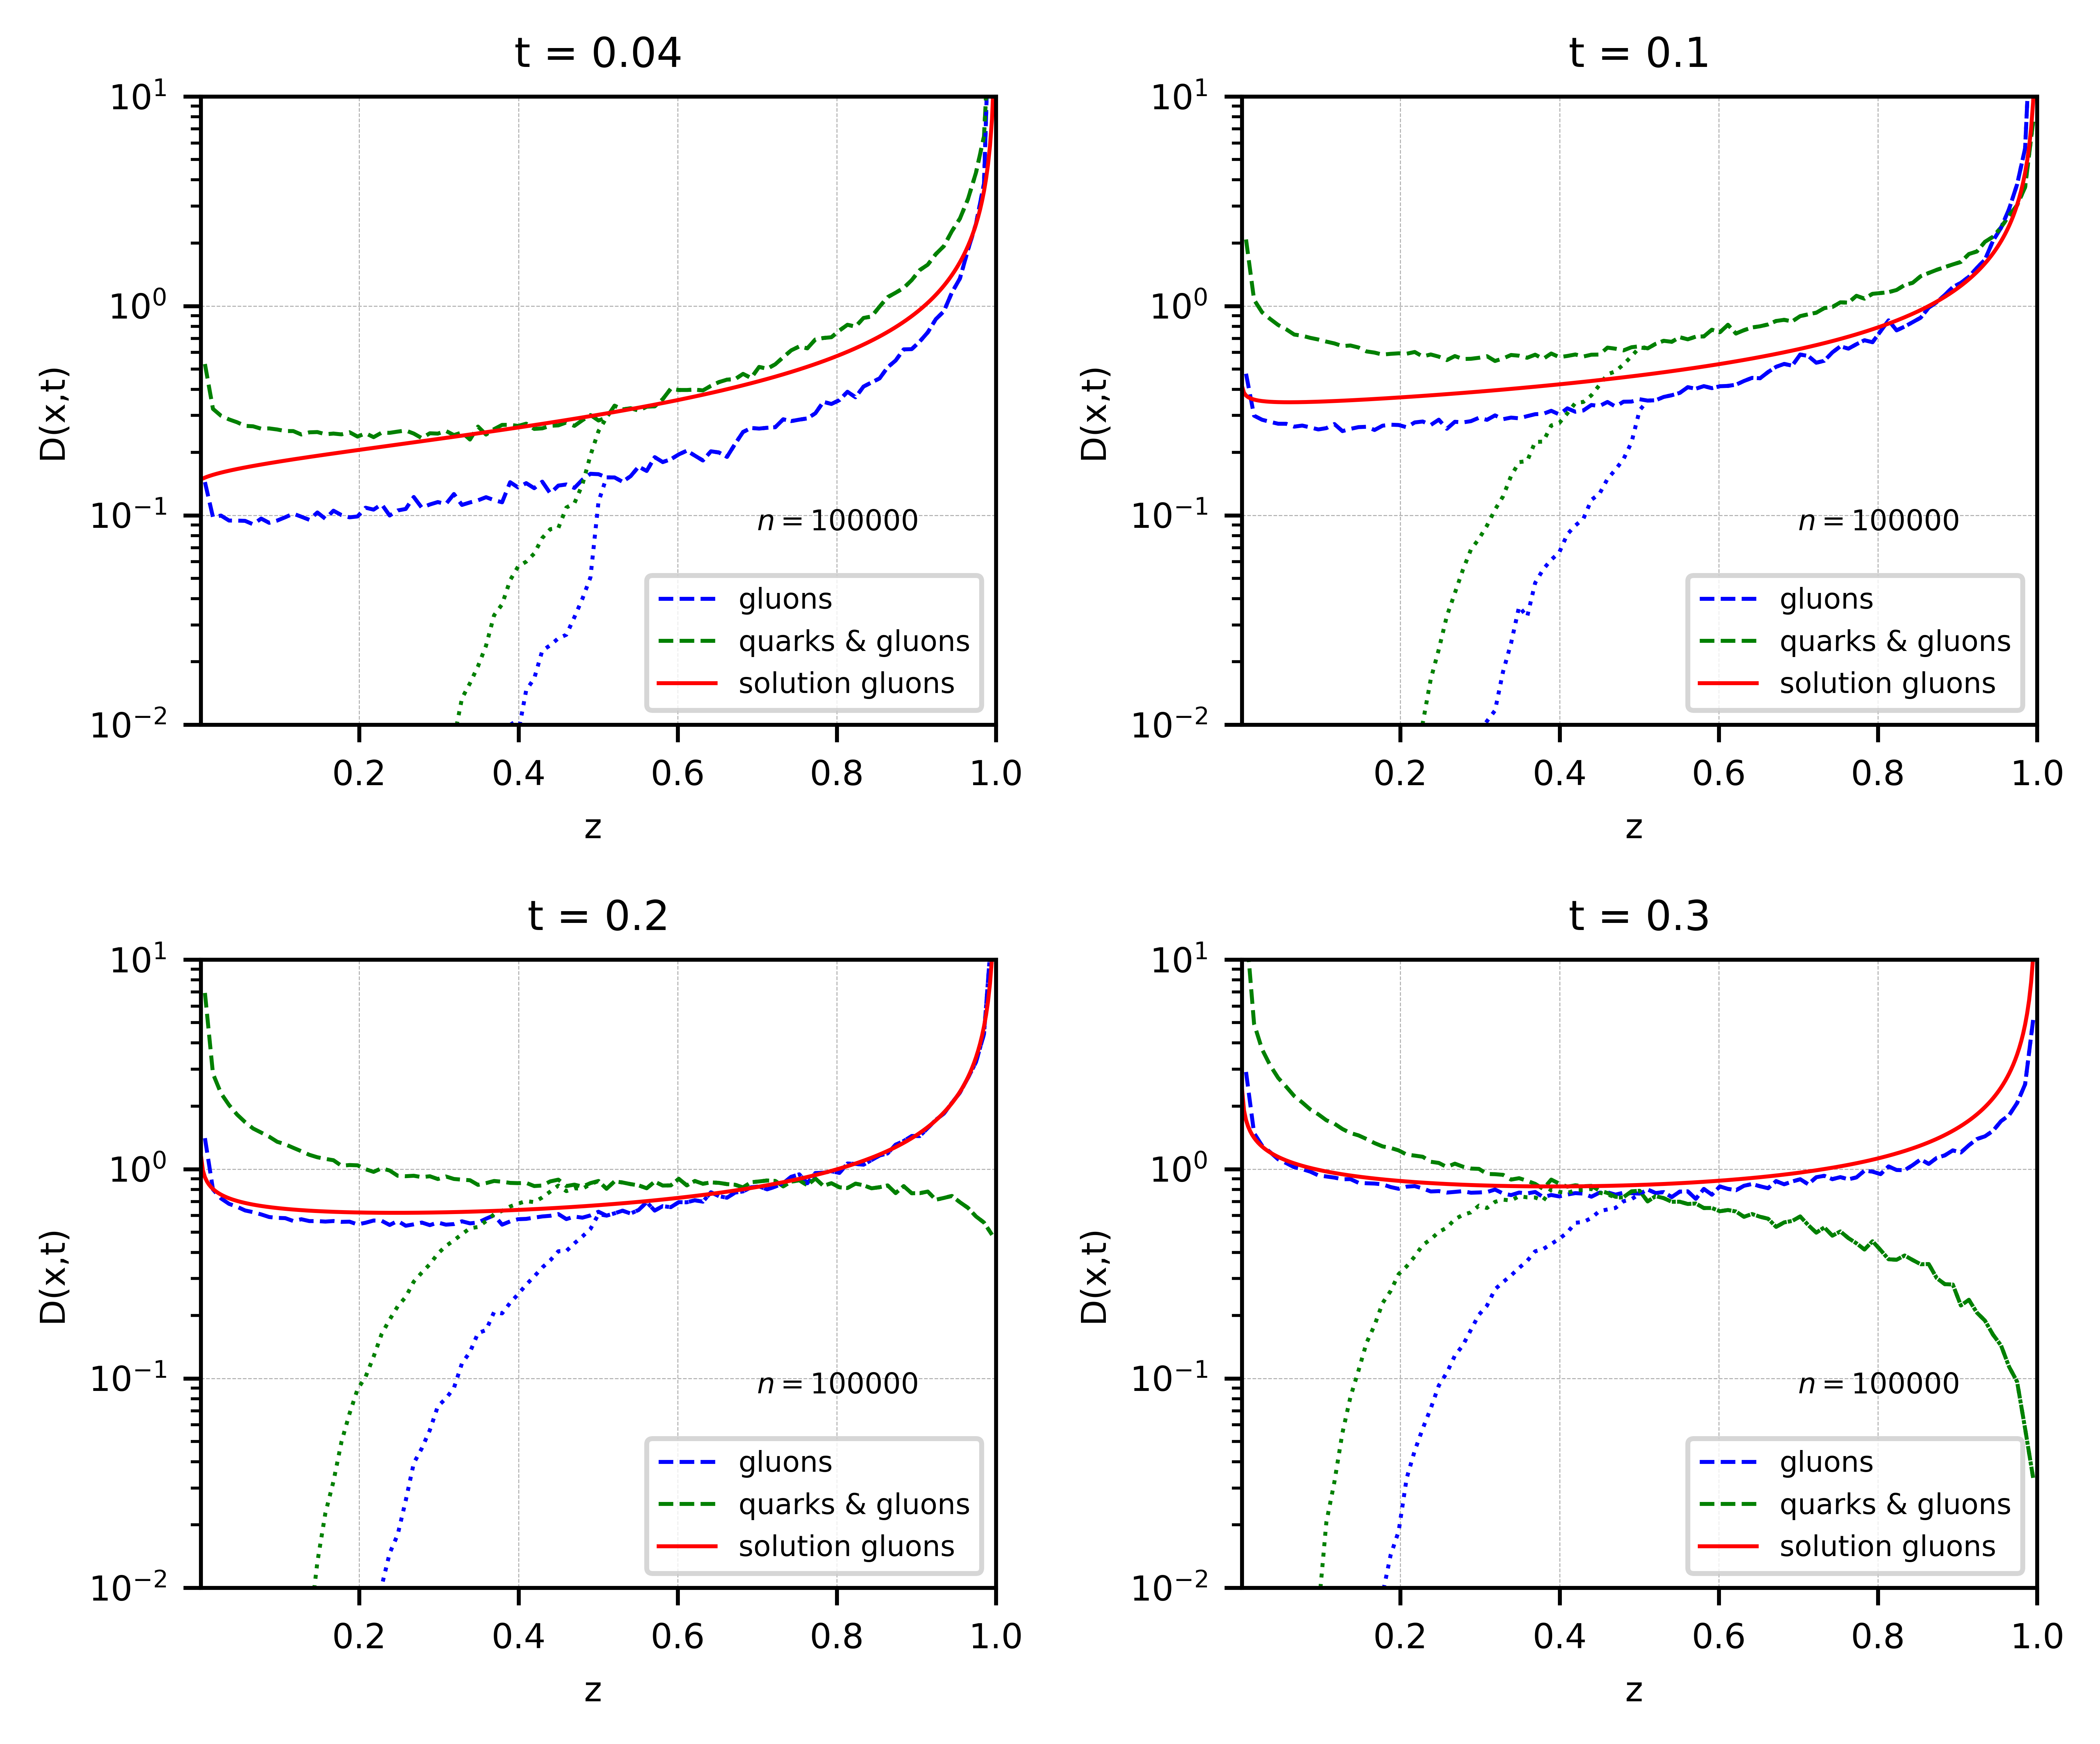
\includegraphics[width=12cm]{pictures/plots/distributions/program_comparison/comparison_vacuum_programs_100k.png}
    \caption{Inclusive spectrum generated from the Monte-Carlo program with gluons only in vacuum, compared to the inclusive spectrum of quarks and gluons in vacuum with the initial parton being a gluon. The red line gives the analytical solution for gluons only. Simulated with \(n = 10^5\) showers, using \(\epsilon=10^{-3}\) and \(z_{\text{min}}=10^{-3}\).}
    \label{fig: vacuum_program_comparisons}
\end{figure}
The plot given here is a straight up comparison of the two programs. It is therefore important to note that the splitting functions are not identical as the gluons only program is using the simplified splitting function which does not carry any color factors. This is apparent when examining the integrals over the different splitting functions, using \(\epsilon = 10{-3}\), 
\begin{align}
\begin{split}
    \int_\epsilon^{1-\epsilon} P_{gg}^{\text{simple}}dz &\approx 13.8\\ \int_\epsilon^{1-\epsilon} P_{gg}^{\text{full}}dz &\approx 36.0\\ \int_\epsilon^{1-\epsilon} P_{qg}^{\text{full}}dz &\approx 1.7 \\
    \int_\epsilon^{1-\epsilon} P_{qq}^{\text{full}}dz &\approx 16.4
\end{split}
\end{align}
Since the expected splitting intervals is inversely proportional to these integrals, it is to be expected that the gluon-only shower using the simplified \(P_{gg}^{\text{simple}}\) splitting function, would be going much slower towards small \(x\) values. If we were to adjust the simplified splitting function such that the expected intervals of \(g\rightarrow gg\) branchings were identical, then the gluon-only distribution would go faster towards low \(x\) values than the gluon initiated showers with both quarks and gluons. There are two reasons for this. The first is that gluons can split using either the \(P_{gg}^{\text{full}}\) or \(P_{qg}^{\text{full}}\) splitting function, the second is that when we inevitably get a \(g\rightarrow q\bar q\) splitting, those new quarks will split much slower than gluons. Both of these properties are direct consequences of how the branching intervals are calculated. 

The difference in color factors does not affect the splitting values in the same manner, as those are calculated by two integrals over the splitting function, meaning the constant factors simply cancel each other out.

\newpage
\section{Monte-Carlo for parton branching in medium}
Moving on to parton branchings in medium. We will be developing a single program in this section which is a Monte-Carlo for the pure gluon cascade. Analogous to the pure gluon cascade in vacuum, we have an analytical solution which we can compare the results with. 

\subsection{Evolution interval}
As discussed in \autoref{sec: BDMPS_theory}, the medium cascade evolves according to the actual time, up to the characteristic time which is the time it takes for the initial parton to radiate most of its energy into soft gluons. This is not necessarily a hard cutoff or boundary for the actual medium cascade, but it is an important property which will affect our expectations for the distributions for different values of \(\tau\). However when developing the Monte-Carlo program it will serve as a guide to which values of \(\tau\) we are interested in.
\begin{align}\label{eqn: medium_evolution_boundaries}
    0 < t &\lessapprox t_* = \frac{\pi}{\alpha_S N_C} \sqrt{\frac{E}{\hat q}} \nonumber \\
    0 < \tau &\lessapprox 1
\end{align}
Determining the probable splitting time can again be done from the Sudakov form factor which was introduced for the medium evolution in \autoref{eqn: BDMPS_sudakov}, and we can therefore follow the procedure of \autoref{sec: determining_evolution_time_from_sudakov} to determine a probable branching interval \(\Delta t = t-t_0\). Doing this in terms of \(\tau\), such that \(\Delta \tau = \Delta t/t_*\), and \(\Delta t/t_*(x) = \Delta t/t_* \sqrt{x} = \Delta \tau/\sqrt{x}\). The evolution probability takes therefore the form,
\begin{align}
    \mathcal{P}(\Delta t) &= \frac{\Delta(t_0)}{\Delta(t)} = \exp \left(- \frac{\Delta t}{t_*(x)} \int_\epsilon^{1-\epsilon} \, dz\, z \mathcal{K}(z) \right) \nonumber \\
    \mathcal{P}(\Delta \tau) &= \frac{\Delta(\tau_0)}{\Delta(\tau)} = \exp \left(- \frac{\Delta \tau}{\sqrt{x}} \int_\epsilon^{1-\epsilon} \, dz\, z \mathcal{K}(z) \right)
\end{align}
Exchanging the probability with a randomly generated number \(\mathcal{R}\in (0,1)\), we obtain
\begin{align}
    \Delta \tau &= -\frac{\sqrt{x}\,\ln(\mathcal{R}) }{\int_\epsilon^{1-\epsilon} \, dz\, z \mathcal{K}(z)} \nonumber \\
    &= -\frac{\sqrt{x}\,\ln(\mathcal{R}) }{\int_\epsilon^{1-\epsilon} \, dz\, z \mathcal{K}(z)} 
\end{align}
from the symmetry of the splitting kernel, we have \(\int_0^1 \, dz\, z \mathcal{K}(z) = \frac{1}{2} \int_0^1 \, dz \mathcal{K}(z)\), and the probable evolution interval can be therefore be determined from \autoref{eqn: BDMPS_probable_branching_interval_tau}.
\begin{equation}\label{eqn: BDMPS_probable_branching_interval_tau}
    \Delta \tau = -\frac{2\, \sqrt{x}\cdot \ln(\mathcal{R}) }{\int_\epsilon^{1-\epsilon} \, dz \mathcal{K}(z)} 
\end{equation}

\subsection{Sampling from the medium splitting functions}
The medium splitting functions was introduced in the previous chapter, and now we will determine appropriate ways of doing random samples. 

\subsubsection*{Sampling from the \(gg\) vertex}
For gluons in medium, it will be sufficient to work with the simplified splitting kernel as presented in \autoref{eqn: ggg_medium_reduced_kernel}. The reasoning is simply that \autoref{eqn: BDMPS_solution_startingpoint} which was the starting point for our analytical solution, is only dependent on the simplified splitting kernel.
It is also worth noting that all factors \(C_A\) are already absorbed into \(\tau\).

The problem of sampling values directly from the splitting function is still present, so returning to \autoref{eqn: probability_density_for_splitting}, we again need to solve \autoref{eqn: energyfraction_function_R}. 
\begin{equation}\tag{\ref{eqn: energyfraction_function_R}}
    \mathcal{R} \cdot \int_\epsilon^{1-\epsilon} dz \, \mathcal{K}(z) = \int_\epsilon^{y}dz \, \mathcal{K}(z)
\end{equation}
The integral can be generally shown to be, 
\begin{align}
    \int_a^b \frac{1}{(z(1-z))^{3/2}}dz &= \left[ \frac{4z-2}{\sqrt{-z(z-1)}} \right]_a^b
\end{align}
which means that we can evaluate \autoref{eqn: energyfraction_function_R} as,
\begin{align}
    \mathcal{R} \int_\epsilon^{1-\epsilon} dz \, \frac{1}{(z(1-z))^{3/2}} &= \int_\epsilon^{y} \frac{1}{(z(1-z))^{3/2}} \nonumber \\
    \mathcal{R} \left(  \frac{4(1-\epsilon)-2}{\sqrt{-(1-\epsilon)((1-\epsilon)-1)}} - \frac{4\epsilon-2}{\sqrt{-\epsilon(\epsilon-1)}} \right) &= \frac{4y-2}{\sqrt{-y(y-1)}} - \frac{4\epsilon-2}{\sqrt{-\epsilon(\epsilon-1)}} \nonumber\\
    \mathcal{R} \left(  \frac{2-4\epsilon}{\sqrt{\epsilon(1-\epsilon)}} - \frac{4\epsilon-2}{\sqrt{\epsilon(1-\epsilon)}} \right) &= \frac{4y-2}{\sqrt{-y(y-1)}} - \frac{4\epsilon-2}{\sqrt{-\epsilon(\epsilon-1)}} \nonumber\\
    \mathcal{R} \left(  \frac{4-8\epsilon}{\sqrt{\epsilon(1-\epsilon)}} \right) - \frac{2-4\epsilon}{\sqrt{\epsilon(1-\epsilon)}} &= \frac{4y-2}{\sqrt{-y(y-1)}} 
\end{align}
The term on the l.h.s can be written in terms of the integral again and assigned to a variable \(a\), 
\begin{equation}
    a = \int_\epsilon^{1-\epsilon} dz \cdot \left(\mathcal{R} - \frac{1}{2} \right) = \mathcal{R} \left(  \frac{4-8\epsilon}{\sqrt{\epsilon(1-\epsilon)}} \right) + \frac{2-4\epsilon}{\sqrt{\epsilon(1-\epsilon)}}
\end{equation}
Inserting this \(a\), the remainder of the equation can be solved using Mathematica,
\begin{align}\label{eqn: medium_gg_sampling}
    y &= \frac{16 + a^2 \mp a \sqrt{16 + a^2}}{2 (16 + a^2)} \nonumber\\
    y &= \frac{1}{2} \mp \frac{a \sqrt{16 + a^2}}{2 (16 + a^2)} \nonumber\\
    y &= \frac{1}{2} \mp \frac{a }{2 \sqrt{16 + a^2}}
\end{align}
And we now have a method for randomly sampling from the simplified splitting kernel. The histogram of the randomly sampled values compared to the exact splitting function is given in \autoref{fig: medium_gg_sampling}. 
\begin{figure}[htb]
    \centering
    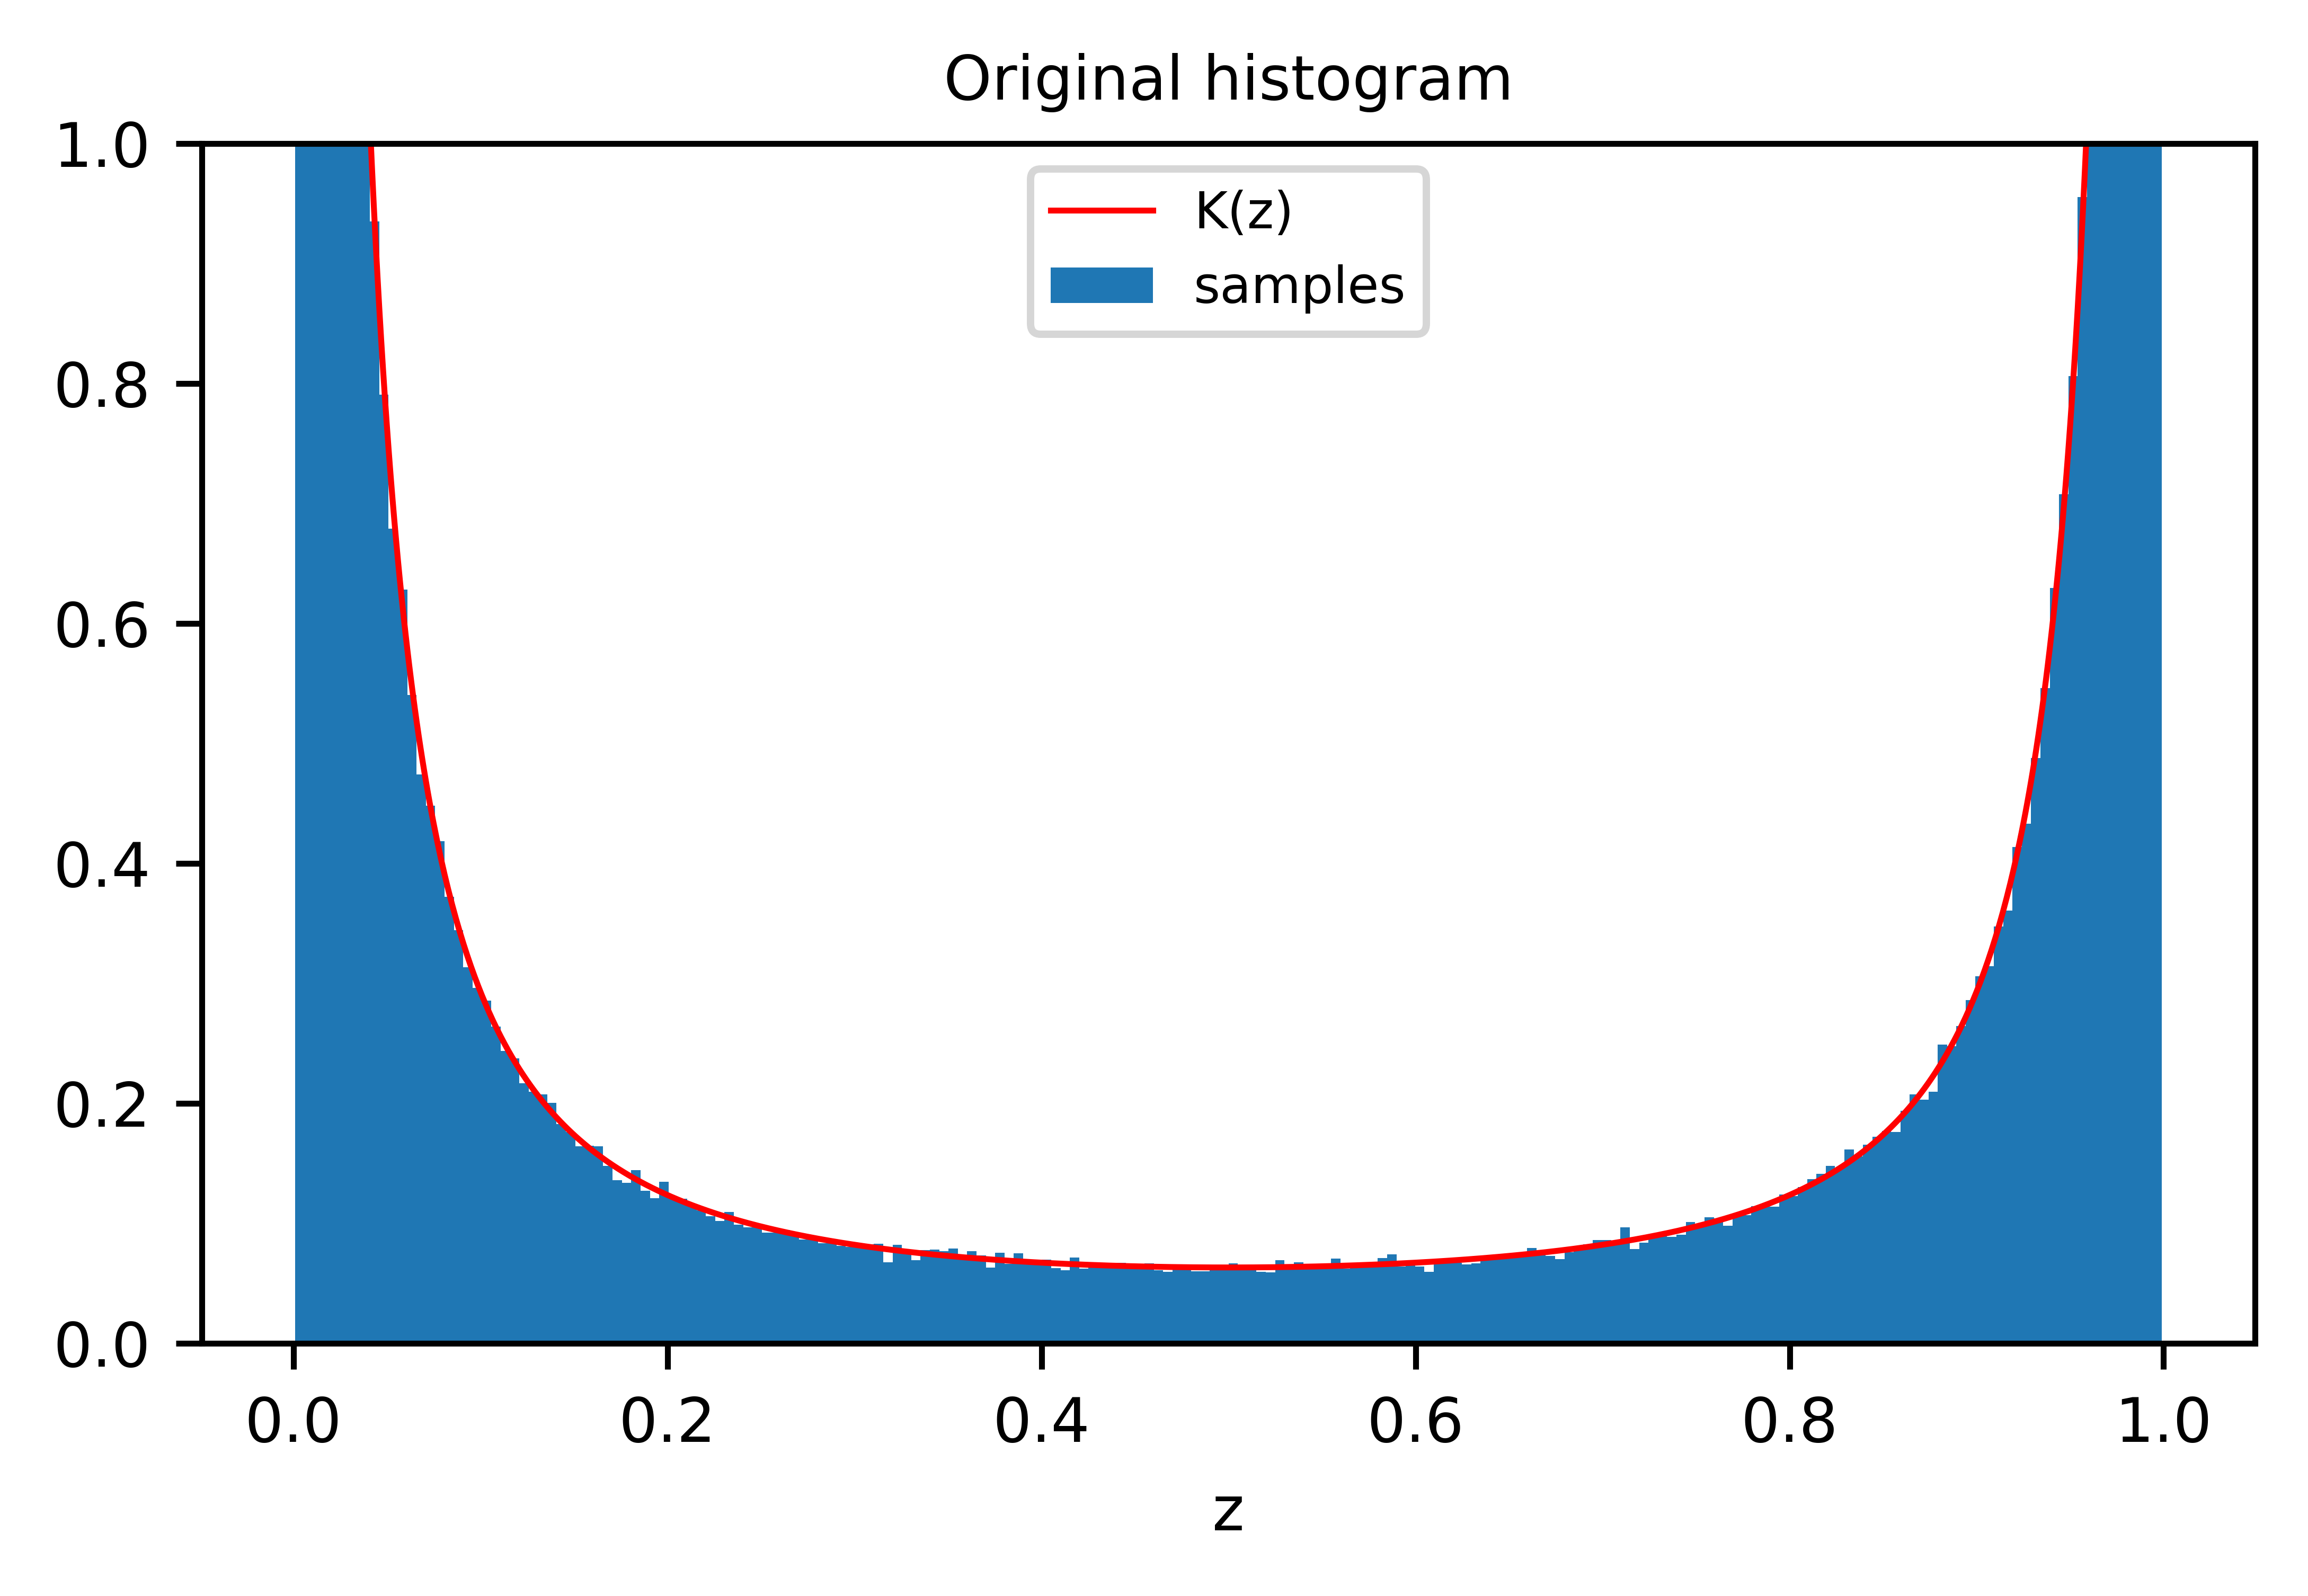
\includegraphics[width=9cm]{pictures/plots/splitting_functions/medium_gg_samples.png}
    \caption{Plot of the simplified kernel \(\mathcal{K}(z)\) for \(gg\) splittings in medium, compared to the sampled values as calculate by \autoref{eqn: medium_gg_sampling}. Total of  \(1,000,000\) samples.}
    \label{fig: medium_gg_sampling}
\end{figure}

\subsection{Monte-Carlo implementation}
Creating the Monte-Carlo program for the medium showers follows generally the same procedure as in vacuum. For now we will restrict ourselves to gluons only, and the simplified splitting kernel. There are some obvious differences, as we now need to generate evolution intervals from the BDMPS sudakov form factor from \autoref{eqn: BDMPS_probable_branching_interval_tau}, and need to sample from the simplified medium splitting kernel \autoref{eqn: medium_gg_sampling}. The other parameters are very similar, and we will need a lower limit on how soft gluon can split. This is particularly important for the medium cascade, as very soft gluons will barely evolve \(\tau\) at all, due to the \(x\) dependence of the generated evolution interval, meaning the program will be incredibly slow. This limit is simply introduced by not appending gluons below a certain limit to the list of splitting gluons. When the plots are made it is then important to keep in mind where this limit is as momentum values below this is not valid. 

The final program is available in the authors GitHub repository \cite{GitHub_thesis}.


\subsection{Results for gluons-only in medium}
This section will be dedicated to verifying the results from out medium showers. Very similar to the vacuum programs we will compare the generated distributions with the analytical solution of the evolution equations, and other properties present will be highlighted using different plots.

We will now plot the inclusive distribution from the Monte-Carlo parton shower, along with the analytical solution for the BDMPS equation as obtained in \autoref{eqn: BDMPS_solution}. It is important to keep in mind that this solution is only valid for the simplified splitting kernel. The resulting plot is given with a linear scale in \autoref{fig: medium_gluoncomparison_analytical}. It is apparent that the Monte-Carlo results are in generally good agreement with the analytical solution. However it does go a bit too slow for higher values of \(z\) for all values of \(\tau\). \krs{how and why}
\begin{figure}[htb]
    \centering
    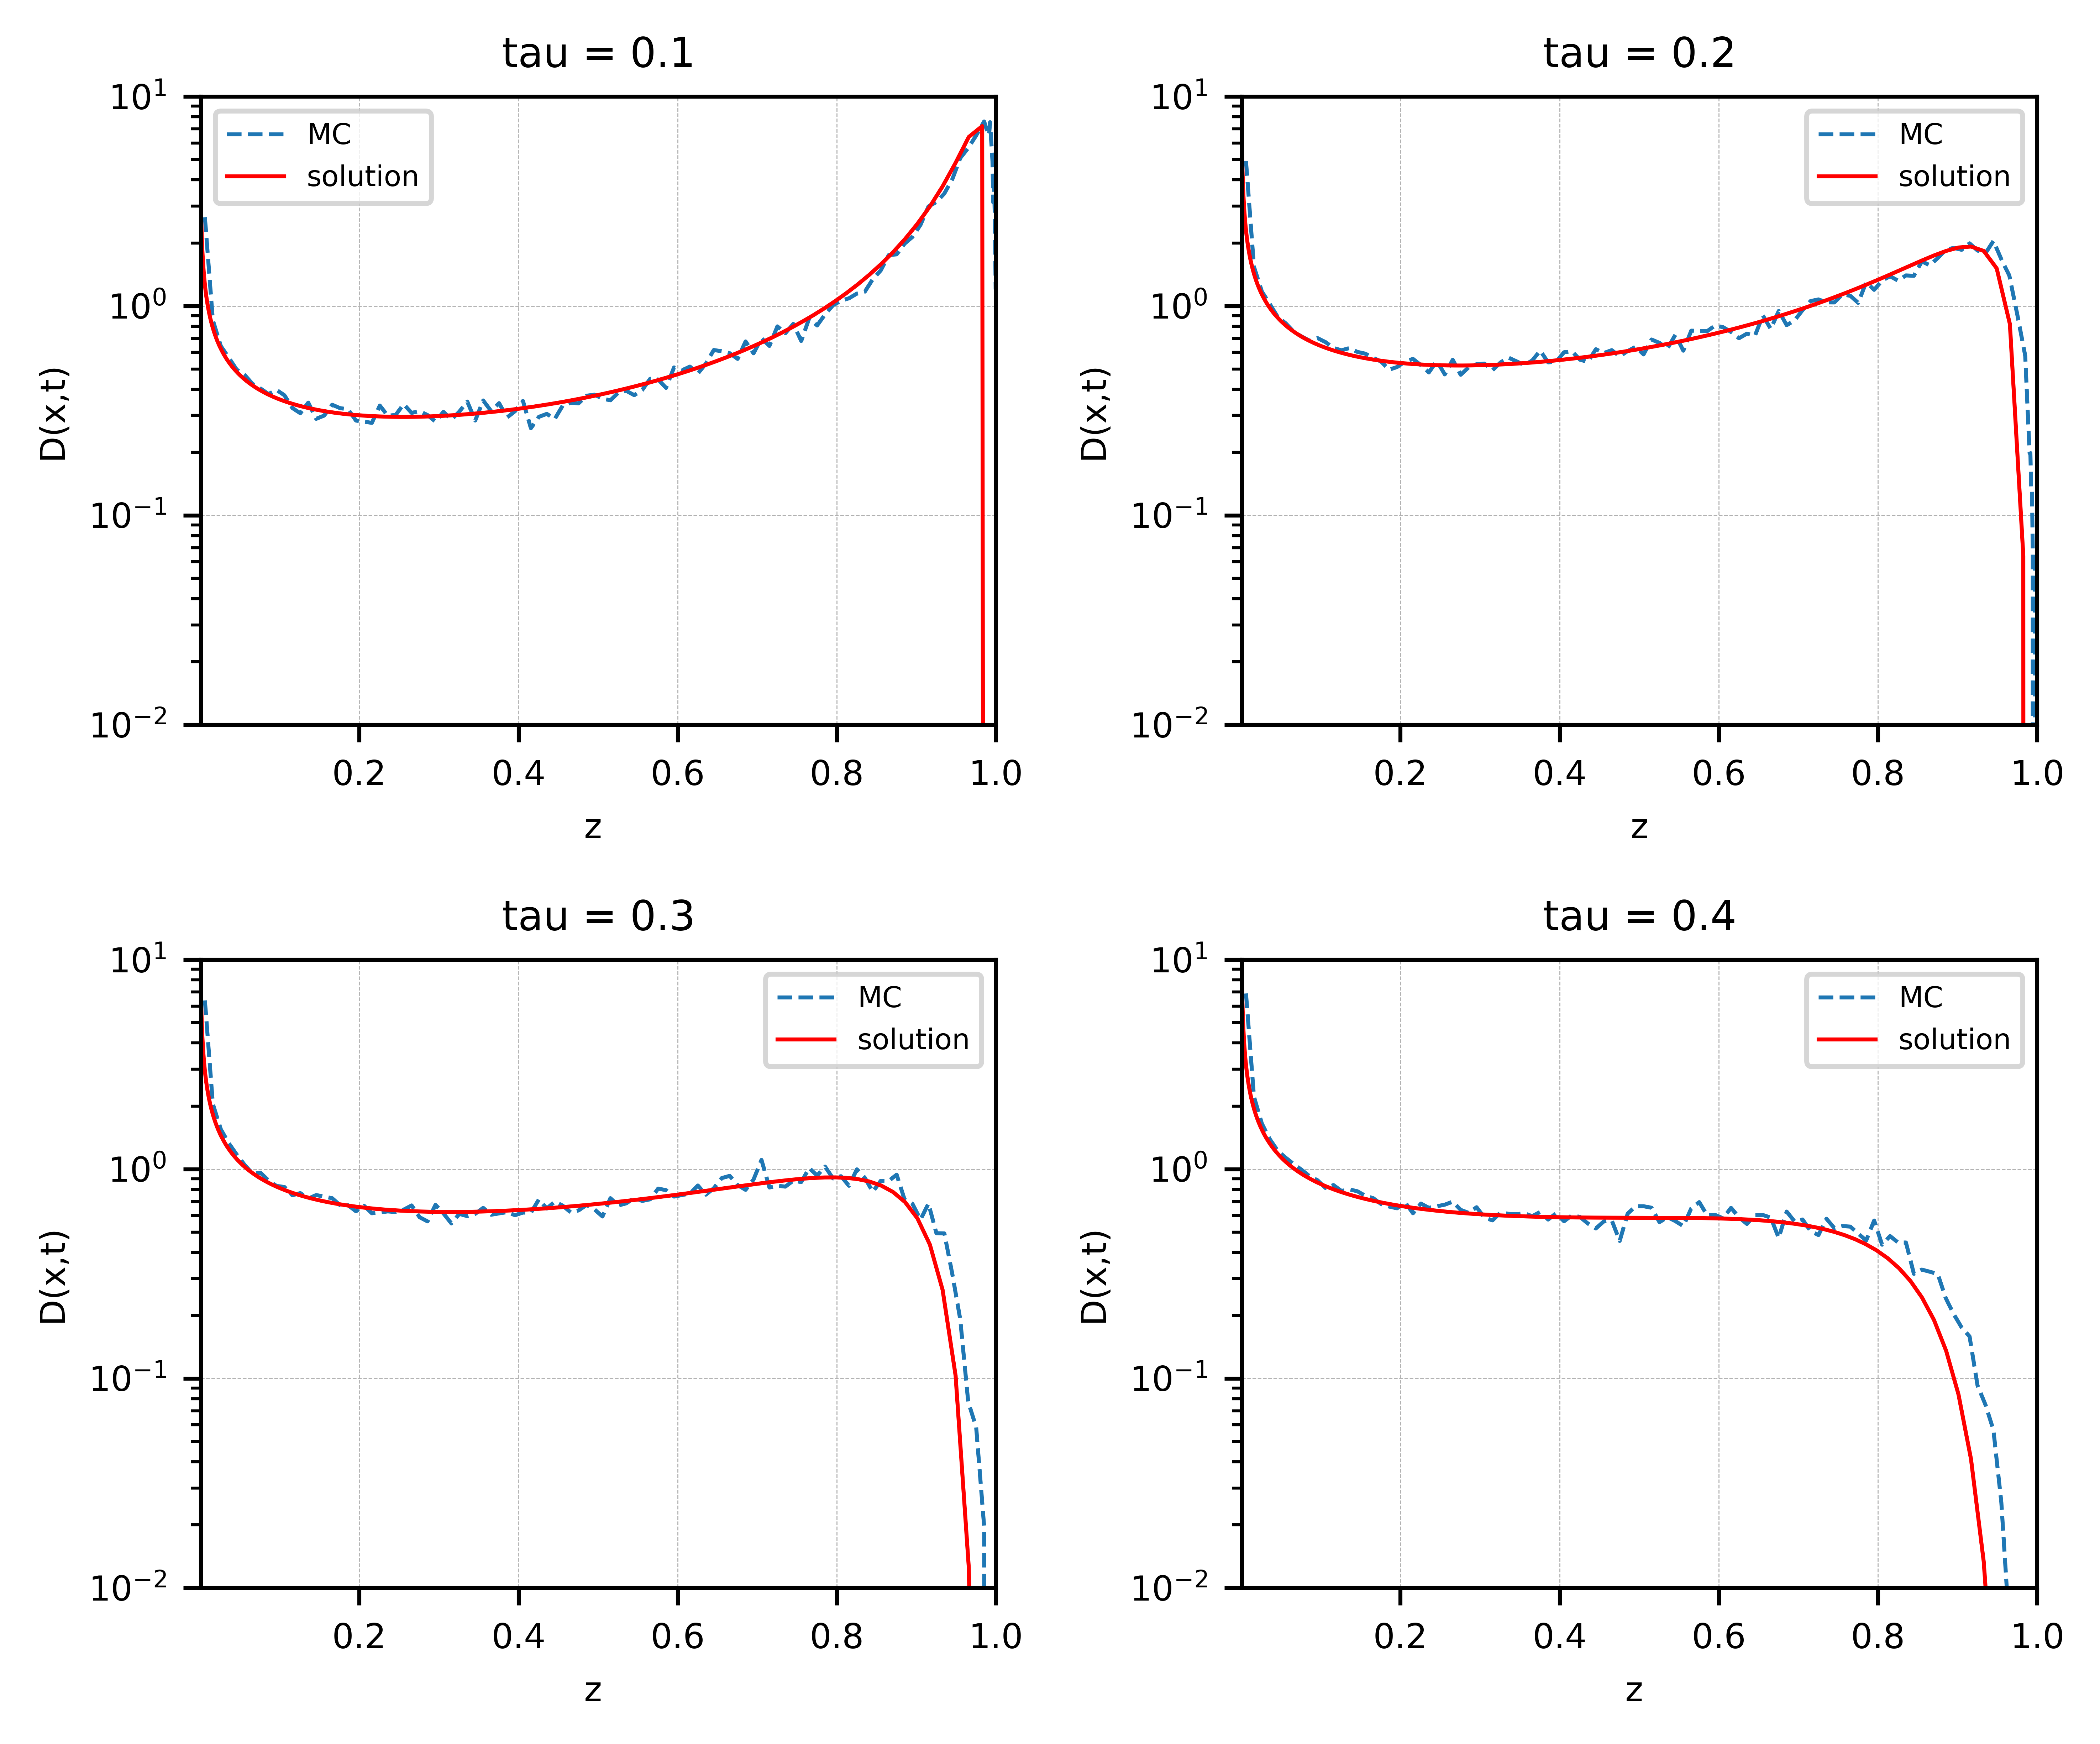
\includegraphics[width=12cm]{pictures/plots/distributions/medium/medium_shower__15k_lin_epsilon3_zmin3_MCandAnalytical.png}
    \caption{Plot of the distribution \(D(x,\tau)\) as generated from the gluons in medium parton shower program using the simplified splitting kernel. Monte-carlo is run for \(15.000\) showers, using \(\epsilon=10^{-3}\) and \(z_{\text{min}} = 10^{-3}\). The distribution is compared with the analytical solution given in \autoref{eqn: BDMPS_solution} and plotted with a lin scale.}
    \label{fig: medium_gluoncomparison_analytical}
\end{figure}

For observing the scaling property of the medium evolution, we will plot the distribution for many different values of \(\tau\). This is presented in \autoref{fig: medium_comparison_scaling}. The scaling properties of the medium evolution is apparent, as once the peak corresponding to the initial parton around \(z=1\) has disappeared, the flow of energy towards small \(x\) values seems to be constant. As we discussed in \autoref{sec: BDMPS_properties}, the distribution changes in a uniform and shape-conserving way, once \(\tau\) goes larger than \(\tau \sim 1\) \krs{???}. 
\begin{figure}[htb]
    \centering
    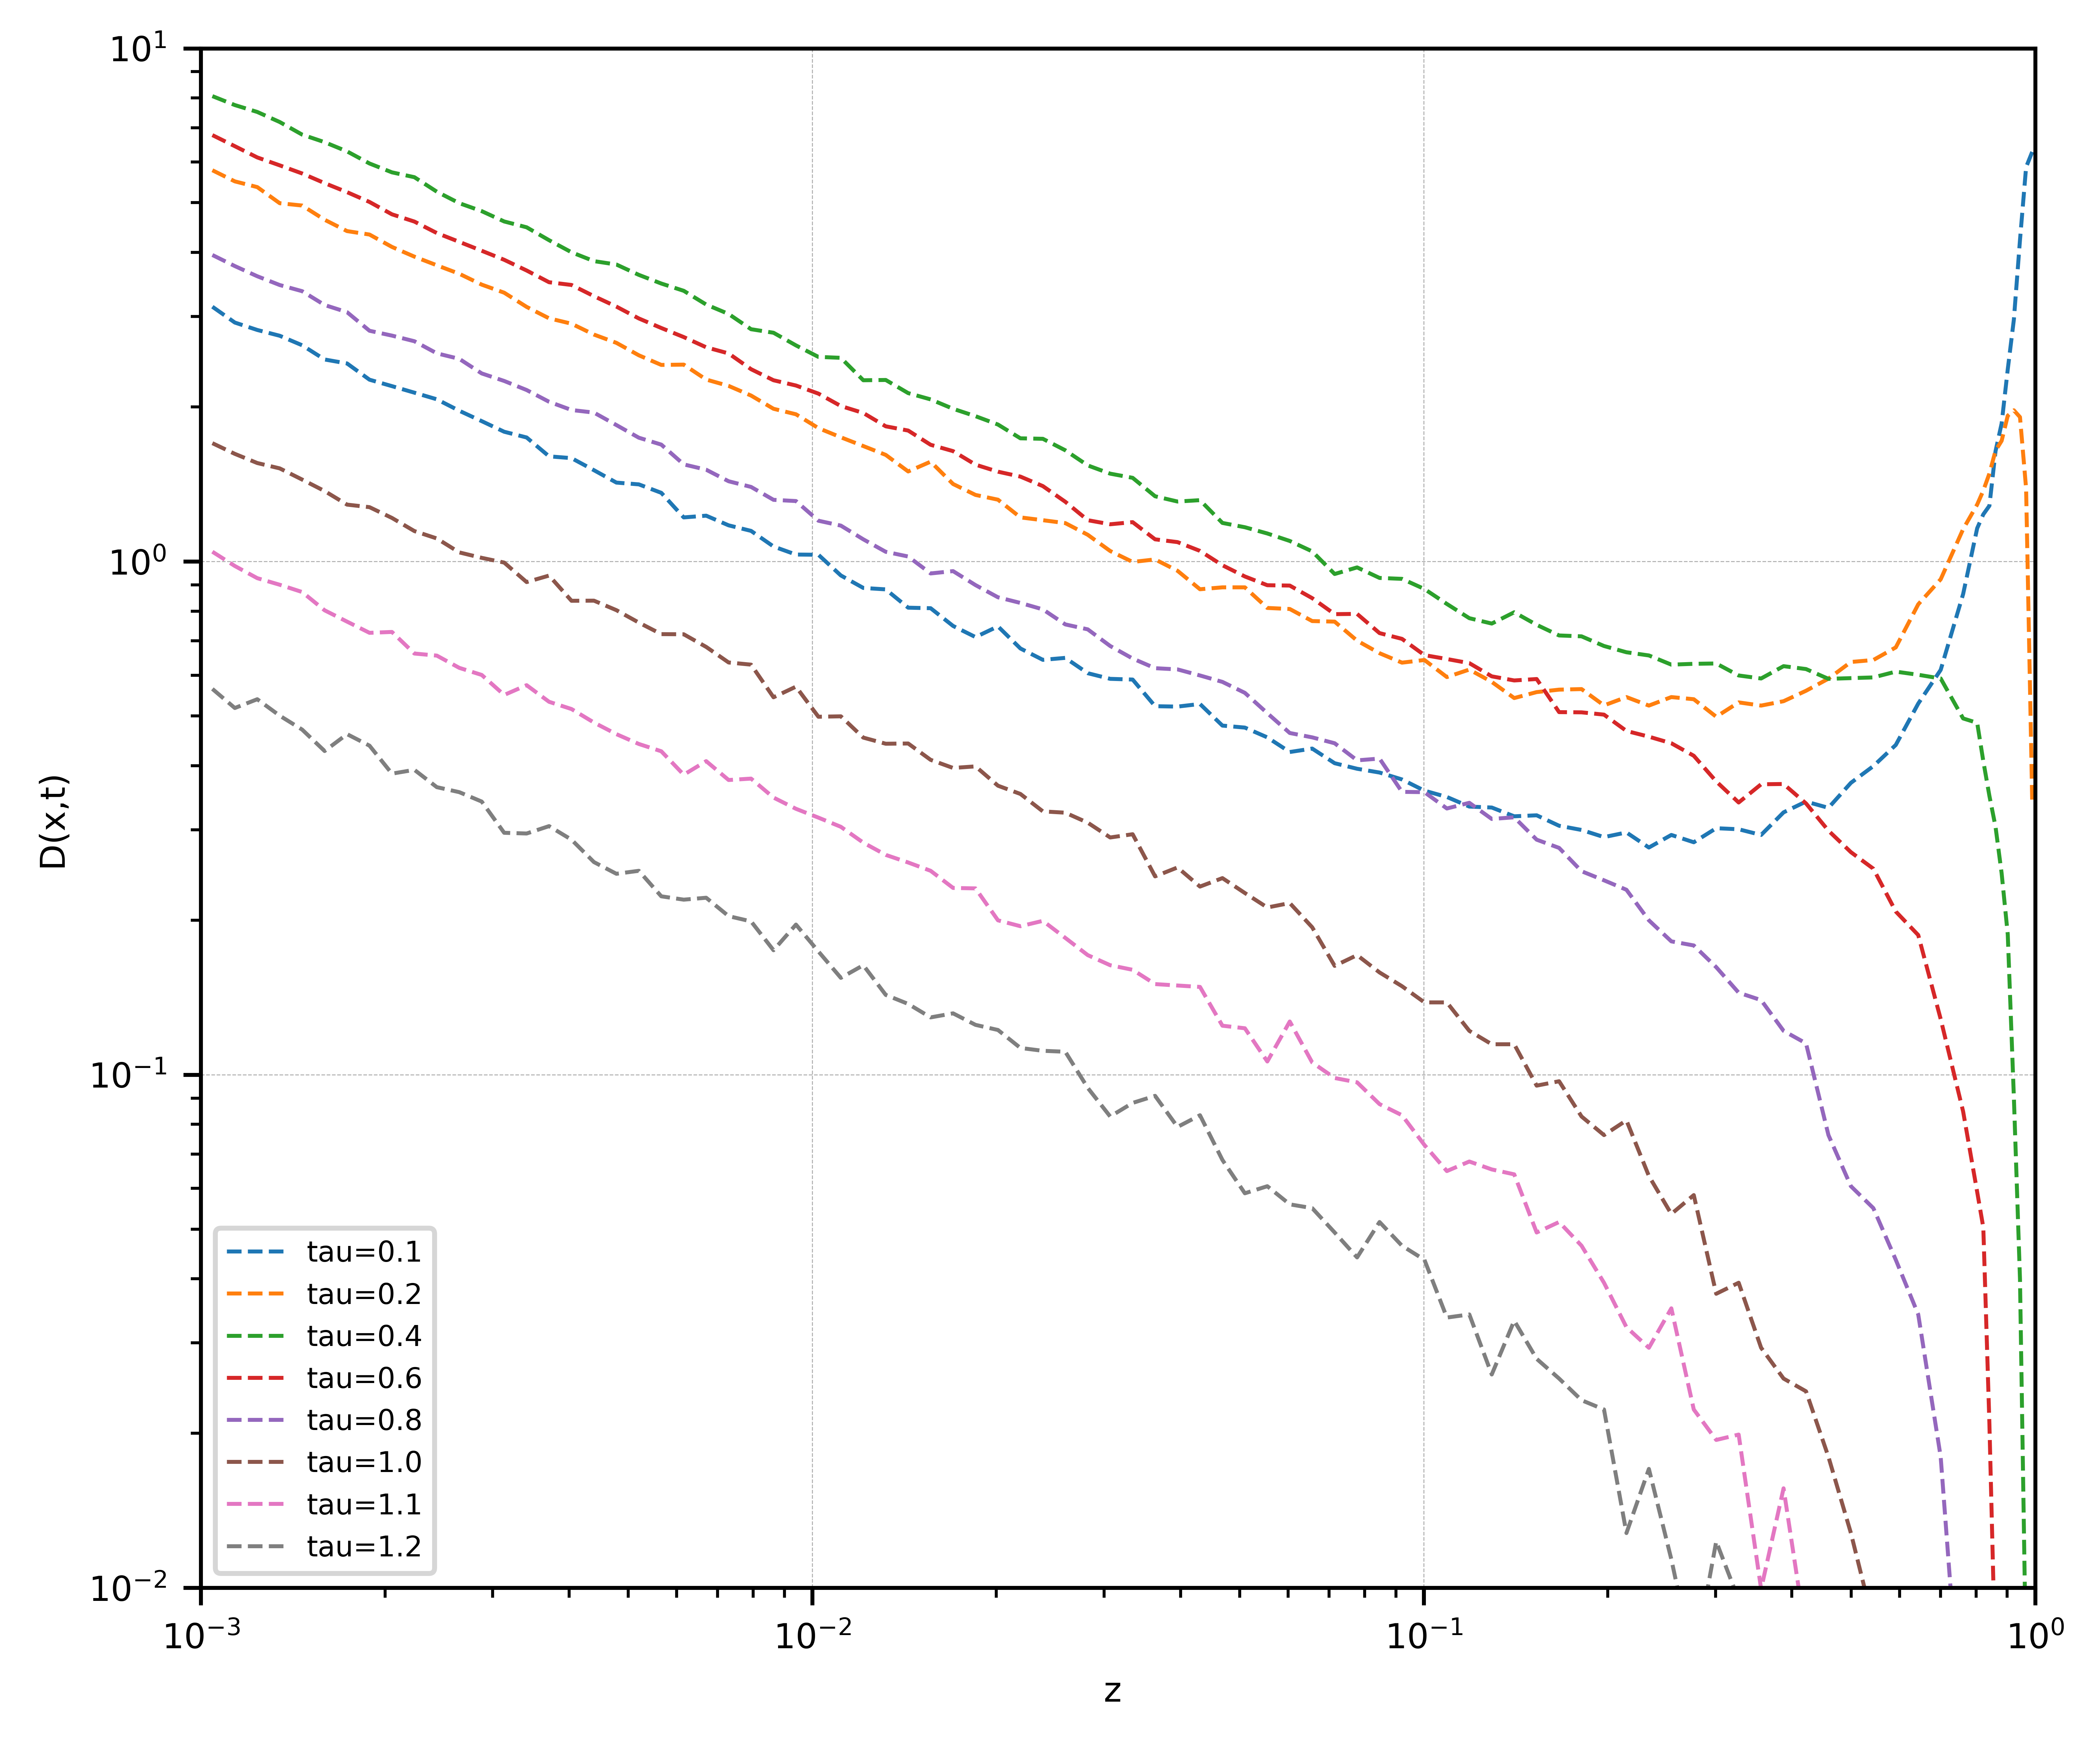
\includegraphics[width=9cm]{pictures/plots/distributions/medium/medium_scaling_25k.png}
    \caption{Plot of the distribution \(D(x,\tau)\) as generated from the gluons in medium parton shower program using the simplified splitting kernel. Monte-carlo is run for \(25.000\) showers, using \(\epsilon=10^{-3}\) and \(z_{\text{min}} = 10^{-3}\), for a wide range of values \(\tau\). The scaling property of the shower is apparent for values of \(\tau > 1\).}
    \label{fig: medium_comparison_scaling}
\end{figure}

\end{document}